\documentclass[11pt,a4paper]{article}

% ---------------------------------------------------------
% PAQUETES DE CONFIGURACIÓN Y ESTILO
% ---------------------------------------------------------
\usepackage[utf8]{inputenc}
\usepackage[T1]{fontenc}
\usepackage{lmodern}
\usepackage[spanish,es-nodecimaldot,es-tabla]{babel}
\usepackage{amsmath, amsfonts, amssymb}
\usepackage{graphicx}
\usepackage{booktabs, tabularx, multirow}
\usepackage{xcolor}
\usepackage{colortbl}
\usepackage{geometry}
\usepackage{fancyhdr}
\usepackage{listings}
\usepackage{float}
\usepackage{caption}
\usepackage{subcaption}
\usepackage{titlesec}
\usepackage{microtype}
\usepackage[most]{tcolorbox}
\usepackage{hyperref}

% Márgenes normalizados de ingeniería
\geometry{
    top=2.5cm,
    bottom=2.5cm,
    left=2.5cm,
    right=2.5cm,
    headheight=15pt
}

% Paleta de colores institucionales y técnicos
\definecolor{unsaacred}{RGB}{140, 20, 20}
\definecolor{unsaacblue}{RGB}{16, 44, 87}
\definecolor{accentteal}{RGB}{13, 148, 136}
\definecolor{alertred}{RGB}{185, 28, 28}
\definecolor{warnamber}{RGB}{217, 119, 6}
\definecolor{tableheader}{RGB}{22, 54, 94}
\definecolor{tablezebra}{RGB}{248, 250, 252}
\definecolor{codegray}{RGB}{247, 248, 250}
\definecolor{codeborder}{RGB}{215, 220, 228}
\definecolor{keywordblue}{RGB}{0, 75, 150}
\definecolor{commentgreen}{RGB}{30, 130, 30}
\definecolor{stringorange}{RGB}{180, 80, 15}

% Configuración de hipervínculos
\hypersetup{
    colorlinks=true,
    linkcolor=unsaacblue,
    citecolor=unsaacred,
    urlcolor=accentteal,
    pdftitle={Informe de Laboratorio: Implementacion y Control de un Brazo Robotico de 6 GDL},
    pdfauthor={Salluca, Choquenaira, Ccasa, Ramos}
}

% Encabezados y pies de página
\pagestyle{fancy}
\fancyhf{}
\fancyhead[L]{\small\textcolor{gray}{\textbf{UNSAAC} · Escuela Profesional de Ingeniería Informática y de Sistemas}}
\fancyhead[R]{\small\textcolor{gray}{Robótica · Brazo Articulado 6 GDL}}
\fancyfoot[L]{\small\textcolor{gray}{Docente: Ing. Jose Mauro Pillco Quispe}}
\fancyfoot[R]{\thepage}
\renewcommand{\headrulewidth}{0.6pt}
\renewcommand{\footrulewidth}{0.4pt}

% Formato de secciones con acentos de color institucional
\titleformat{\section}
  {\normalfont\Large\bfseries\color{unsaacblue}}{\thesection.}{0.7em}{}[\color{unsaacblue}\titlerule]
\titleformat{\subsection}
  {\normalfont\large\bfseries\color{unsaacred}}{\thesubsection.}{0.5em}{}
\titleformat{\subsubsection}
  {\normalfont\normalsize\bfseries\color{unsaacblue}}{\thesubsubsection.}{0.5em}{}

% Cajas de texto destacadas (tcolorbox)
\newtcolorbox{alertaincidente}[1][]{
  colback=red!5!white,
  colframe=alertred,
  fonttitle=\bfseries\color{white},
  title={Incidencia Crítica de Laboratorio: #1},
  arc=3mm,
  boxrule=1.2pt,
  left=8pt, right=8pt, top=8pt, bottom=8pt
}

\newtcolorbox{notatecnica}[1][]{
  colback=blue!5!white,
  colframe=unsaacblue,
  fonttitle=\bfseries\color{white},
  title={Especificación Técnica: #1},
  arc=3mm,
  boxrule=1.2pt,
  left=8pt, right=8pt, top=8pt, bottom=8pt
}

\newtcolorbox{estadolaboratorio}[1][]{
  colback=teal!5!white,
  colframe=accentteal,
  fonttitle=\bfseries\color{white},
  title={Estado Actual en Laboratorio (v2): #1},
  arc=3mm,
  boxrule=1.2pt,
  left=8pt, right=8pt, top=8pt, bottom=8pt
}

% Configuración de listings para código fuente
\lstset{
    backgroundcolor=\color{codegray},
    frame=single,
    rulecolor=\color{codeborder},
    basicstyle=\ttfamily\scriptsize,
    keywordstyle=\color{keywordblue}\bfseries,
    commentstyle=\color{commentgreen}\itshape,
    stringstyle=\color{stringorange},
    numbers=left,
    numberstyle=\tiny\color{gray},
    numbersep=6pt,
    breaklines=true,
    breakatwhitespace=true,
    tabsize=2,
    showstringspaces=false,
    captionpos=b,
    inputencoding=utf8,
    extendedchars=true,
    literate={á}{{\'a}}1 {é}{{\'e}}1 {í}{{\'i}}1 {ó}{{\'o}}1 {ú}{{\'u}}1 {ñ}{{\~n}}1 {°}{{$^\circ$}}1
}

% ---------------------------------------------------------
% CUERPO DEL INFORME
% ---------------------------------------------------------
\begin{document}

% =========================================================
% PORTADA INSTITUCIONAL (MODELO UNSAAC EXACTO)
% =========================================================
\begin{titlepage}
    \centering
    {\bfseries\large UNIVERSIDAD NACIONAL DE SAN ANTONIO ABAD DEL CUSCO}\\[0.25cm]
    {\bfseries\normalsize FACULTAD DE INGENIERÍA ELÉCTRICA,\\ELECTRÓNICA, INFORMÁTICA Y MECÁNICA}\\[0.25cm]
    {\bfseries\normalsize ESCUELA PROFESIONAL DE INGENIERÍA INFORMÁTICA\\Y DE SISTEMAS}\\[0.8cm]
    
    
\includegraphics[width=0.30\textwidth]{img/escudo.png}\\[0.9cm]
    
    \hrule height 1.2pt
    \vspace{0.4cm}
    {\bfseries\Large IMPLEMENTACIÓN Y CONTROL DE UN BRAZO ROBÓTICO ARTICULADO DE 6 GDL}\\[0.4cm]
    \hrule height 1.2pt
    
    \vspace{1.2cm}
    
    \begin{flushleft}
    \textbf{Asignatura:} ROBÓTICA\\[0.25cm]
    \textbf{Docente:} Ing. Jose Mauro Pillco Quispe\\[0.25cm]
    \textbf{Semestre:} 2026-II\\[0.25cm]
    \textbf{Integrantes:}\\[0.15cm]
    \hspace*{0.5cm}\begin{tabular}{p{9.5cm} r}
    \textbullet{} Salluca Chile, Sandro Alexander & \\
    \textbullet{} Choquenaira Quispe, Noe Franklin & \\
    \textbullet{} Ccasa Ccahuana, Flor Deliz & \\
    \end{tabular}
    \end{flushleft}
    
    \vfill
    {\bfseries Cusco -- Perú}\\[0.15cm]
    {\bfseries 2026}
\end{titlepage}

% =========================================================
% ÍNDICE GENERAL
% =========================================================
\tableofcontents
\newpage

% =========================================================
% RESUMEN EJECUTIVO
% =========================================================
\section*{Resumen Ejecutivo}
\addcontentsline{toc}{section}{Resumen Ejecutivo}

El presente informe técnico documenta el diseño, reconfiguración mecatrónica, ensamble estructural y desarrollo de firmware para un \textbf{brazo robótico articulado de seis grados de libertad (6 GDL)}. Siguiendo las directrices del docente de la asignatura, el sistema fue rediseñado sustituyendo los servomotores iniciales por actuadores digitales de alto par torsor (\textbf{45~kg}, \textbf{40~kg} y \textbf{35~kg}), capaces de soportar los momentos estáticos generados por la masa acumulada del manipulador.

En este documento se expone con rigurosidad el estado de avance real del proyecto:
\begin{itemize}
    \item \textbf{Ensamble Mecánico y Diagnóstico de Rigidez:} Se completó el montaje de los 6 grados de libertad sobre una base rígida de madera. Durante las primeras pruebas de elevación, se detectó una falla mecánica crítica: el brazo pierde sustentación y se desploma hacia adelante. La inspección visual determinó que el servocuerno de aluminio carece del tornillo central de apriete axial M3 sobre el eje estriado del servomotor negro de 45~kg (D2450ST), lo que ocasiona deslizamiento mecánico sin transmisión de par ni rigidez en la articulación del hombro.
    \item \textbf{Estado del Conexionado Eléctrico:} Se deja constancia de que el microcontrolador \textbf{ESP32-CAM} y el controlador PWM \textbf{PCA9685} \textbf{aún no han sido conectados físicamente ni energizados}; se diseñó la topología circuital de masa común y aislamiento de rieles para su ejecución en la próxima sesión.
    \item \textbf{Firmware Embebido:} Se presenta y analiza el código fuente íntegro en C++ (\texttt{brazoR.ino}), el cual incorpora servidor HTTP embebido, comunicación $I^2C$ a 50~Hz, algoritmos de movimiento suave e interrupción de seguridad (\textit{watchdog} por inactividad).
\end{itemize}

\vspace{0.4cm}
\noindent\textbf{Palabras clave:} Brazo Robótico, 6 GDL, ESP32-CAM, PCA9685, Servomotores de Alto Par, Análisis de Falla Mecánica, UNSAAC.

\newpage

% =========================================================
% SECCIÓN 1
% =========================================================
\section{Introducción y Objetivos}

La robótica manipuladora serial constituye uno de los pilares formativos esenciales en la ingeniería mecatrónica e informática. Los brazos articulados de cadena cinemática abierta presentan retos considerables en el balance entre la rigidez estructural, la densidad de potencia de los actuadores y la precisión temporal en la modulación de señales de control.

\subsection{Objetivos del Laboratorio}
\begin{itemize}
    \item \textbf{Objetivo General:} Implementar, ensamblar y programar un manipulador robótico de 6 grados de libertad teleoperado de manera inalámbrica mediante un microcontrolador ESP32-CAM y un controlador PWM periférico PCA9685.
    \item \textbf{Objetivos Específicos:}
    \begin{enumerate}
        \item Reemplazar los actuadores convencionales por servomotores digitales de alto par torsor (45~kg, 40~kg y 35~kg) para satisfacer el balance estático del manipulador.
        \item Identificar y diagnosticar mediante inspección visual las holguras mecánicas y pérdidas de rigidez en las uniones hombro y codo.
        \item Diseñar un esquema circuital con aislamiento estricto entre el riel de alimentación lógica y el riel de potencia de los motores.
        \item Desarrollar y verificar el firmware en C++ para el microcontrolador ESP32-CAM con servidor web embebido y parada de emergencia.
    \end{enumerate}
\end{itemize}

% =========================================================
% SECCIÓN 2
% =========================================================
\section{Arquitectura General del Sistema y Hardware}

El manipulador robótico antropomórfico está compuesto por tres subsistemas interconectados: subsistema mecánico, subsistema de control electrónico y subsistema de comunicaciones.

\subsection{Distribución Cinemática de los 6 Grados de Libertad (6 GDL)}
Cada eje de rotación cumple un rol geométrico determinado dentro del espacio de trabajo del efector final:
\begin{enumerate}
    \item \textbf{Articulación 1 (Base - Azimuth):} Rotación sobre el plano horizontal para cobertura de $120^\circ$.
    \item \textbf{Articulación 2 (Hombro - Pitch):} Elevación del brazo principal contra el vector de gravedad.
    \item \textbf{Articulación 3 (Codo - Pitch):} Posicionamiento radial del antebrazo respecto a la base.
    \item \textbf{Articulación 4 (Muñeca 1 - Pitch):} Inclinación vertical del cabezal de agarre.
    \item \textbf{Articulación 5 (Muñeca 2 - Roll):} Giro axial de la pinza sobre su propio eje.
    \item \textbf{Articulación 6 (Pinza - Gripper):} Prensión mecánica de objetos mediante mordazas paralelas.
\end{enumerate}

\subsection{Plataforma de Procesamiento: ESP32-CAM}
El módulo ESP32-CAM integra un procesador de 32 bits Xtensa dual-core a 240~MHz con Wi-Fi 802.11 b/g/n y Bluetooth integrados. Previo al cableado de periféricos, se verificó el enlace USB-Serial con la base programadora ESP32-CAM-MB en el puerto \texttt{COM7} de Windows, confirmando la operatividad del silicio (Figura~\ref{fig:hardware_base}).

\begin{figure}[H]
    \centering
    \begin{subfigure}[b]{0.48\textwidth}
        \centering
        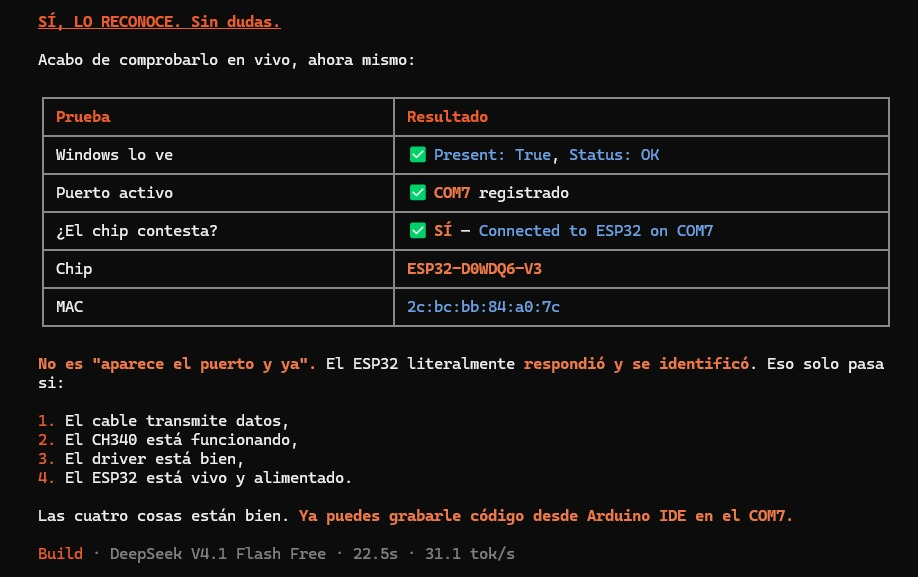
\includegraphics[width=\linewidth, height=6.2cm, keepaspectratio=false]{img/esp32_verificacion_com7.jpeg}
        \caption{Diagnóstico UART: ESP32 en COM7 (MAC confirmada).}
        \label{fig:com7_diag}
    \end{subfigure}
    \hfill
    \begin{subfigure}[b]{0.48\textwidth}
        \centering
        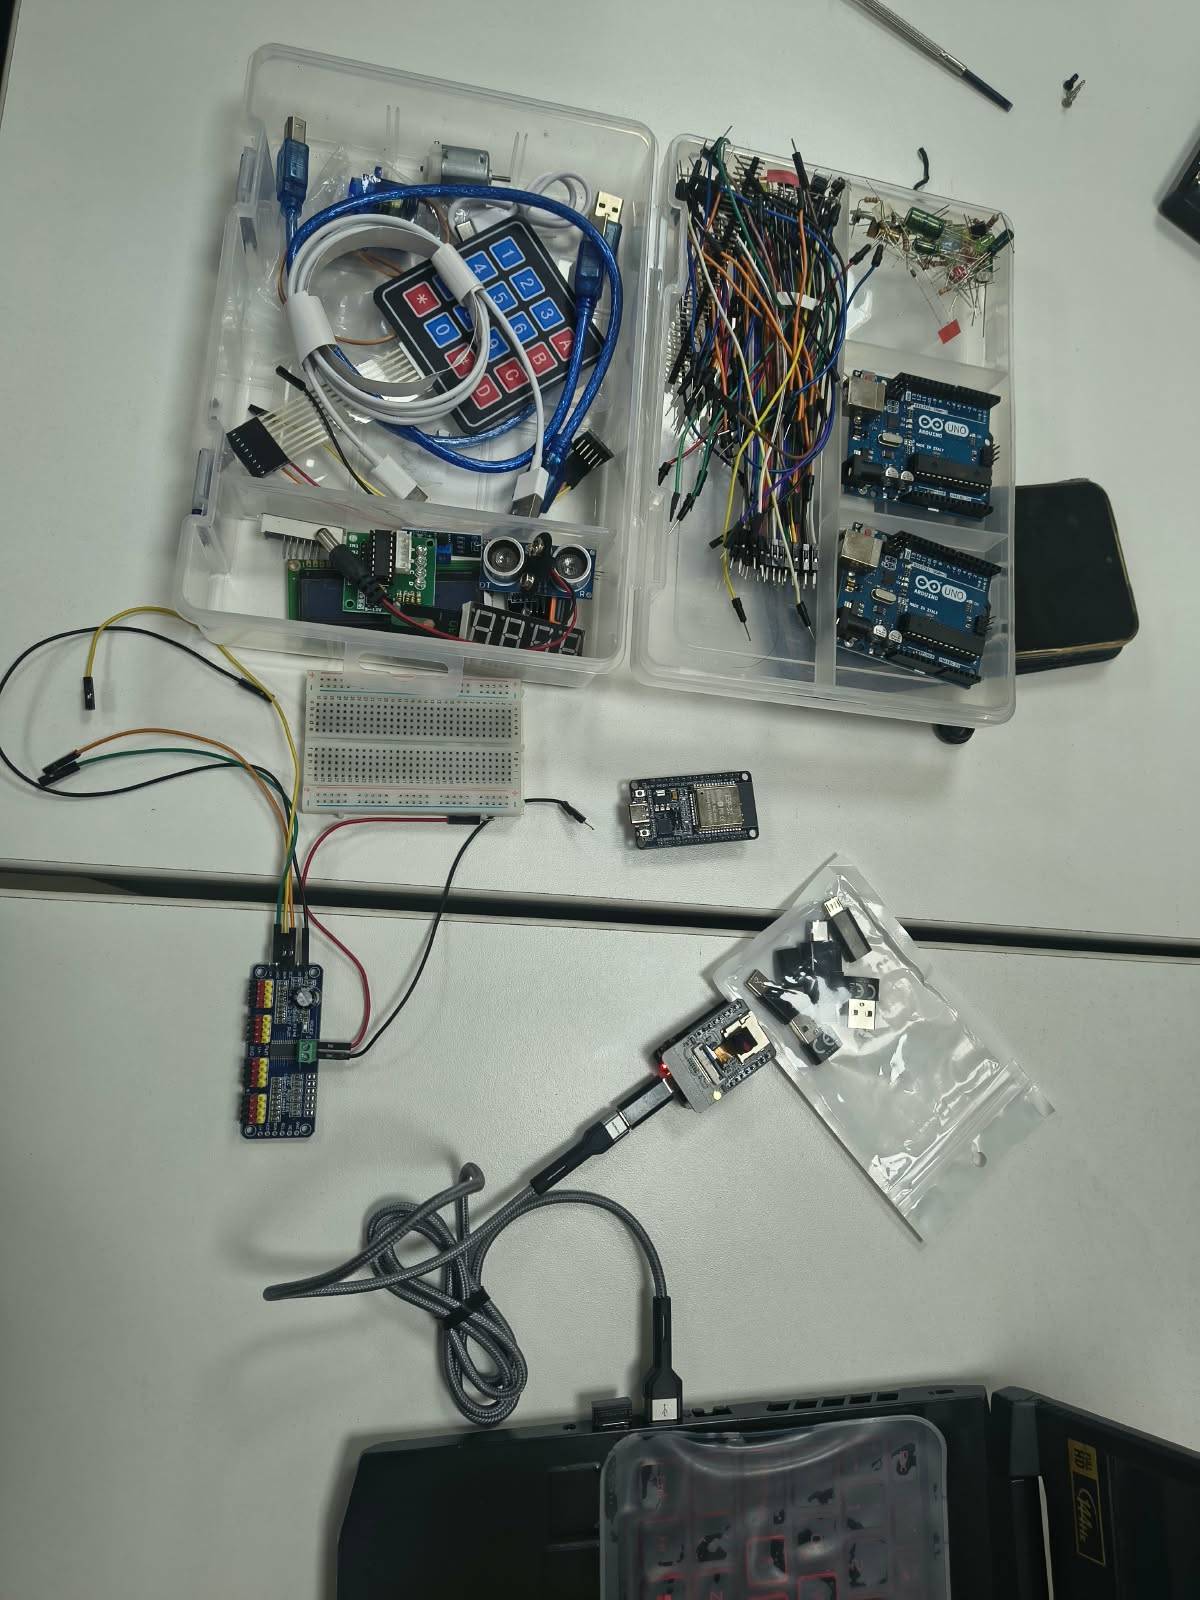
\includegraphics[width=\linewidth, height=6.2cm, keepaspectratio=false]{img/banco_pruebas_electronica.jpeg}
        \caption{Banco de pruebas: instrumentación y componentes.}
        \label{fig:mesa_trabajo}
    \end{subfigure}
    \caption{Verificación instrumental del microcontrolador y banco de trabajo en laboratorio.}
    \label{fig:hardware_base}
\end{figure}

% =========================================================
% SECCIÓN 3
% =========================================================
\section{Análisis y Selección de Servomotores de Alto Par}

El cálculo del momento flector estático en la unión del hombro ($J_2$) demostró que los motores estándar de $10\text{ kg}\cdot\text{cm}$ entraban en zona de bloqueo térmico. Siguiendo las instrucciones del docente, se reconfiguraron los actuadores según la solicitación mecánica de cada eslabón:

\begin{table}[H]
\centering
\caption{Especificaciones Técnicas de los Servomotores Seleccionados}
\label{tab:especificaciones_servos}
\small
\begin{tabularx}{\textwidth}{p{3.0cm} p{2.8cm} p{2.5cm} X}
\toprule
\rowcolor{tableheader}
\textcolor{white}{\textbf{Ubicación}} & \textcolor{white}{\textbf{Modelo}} & \textcolor{white}{\textbf{Tensión / Señal}} & \textcolor{white}{\textbf{Par Torsor y Características}} \\
\midrule
\textbf{Eje 1: Base} & DSSERVO 40~kg & DC 4.8V--6.8V & $\ge 40\text{ kg}\cdot\text{cm}$, piñonería de acero sobre rodamiento axial. \\
\rowcolor{tablezebra}
\textbf{Eje 2: Hombro} & D2450ST 45~kg & DC 4.8V--7.4V & $\ge 45\text{ kg}\cdot\text{cm}$, carcasa con aletas fresadas de disipación. \\
\textbf{Eje 3: Codo} & DSSERVO 40~kg & DC 4.8V--6.8V & $\ge 40\text{ kg}\cdot\text{cm}$, disipador fucsia, anclaje a eslabón tubular. \\
\rowcolor{tablezebra}
\textbf{Eje 4: Muñeca 1} & YSD035 35~kg Digital & DC 4.8V--6.0V & $\ge 35\text{ kg}\cdot\text{cm}$, placa anodizada azul, rango 500--2500~$\mu$s. \\
\textbf{Eje 5: Muñeca 2} & Digital 35~kg & DC 4.8V--6.0V & Giro axial del cabezal en soporte metálico. \\
\rowcolor{tablezebra}
\textbf{Eje 6: Pinza} & Metal Gear Mini & DC 4.8V--6.0V & Transmisión por doble engranaje para mordazas. \\
\bottomrule
\end{tabularx}
\end{table}

\begin{figure}[H]
    \centering
    \begin{subfigure}[b]{0.31\textwidth}
        \centering
        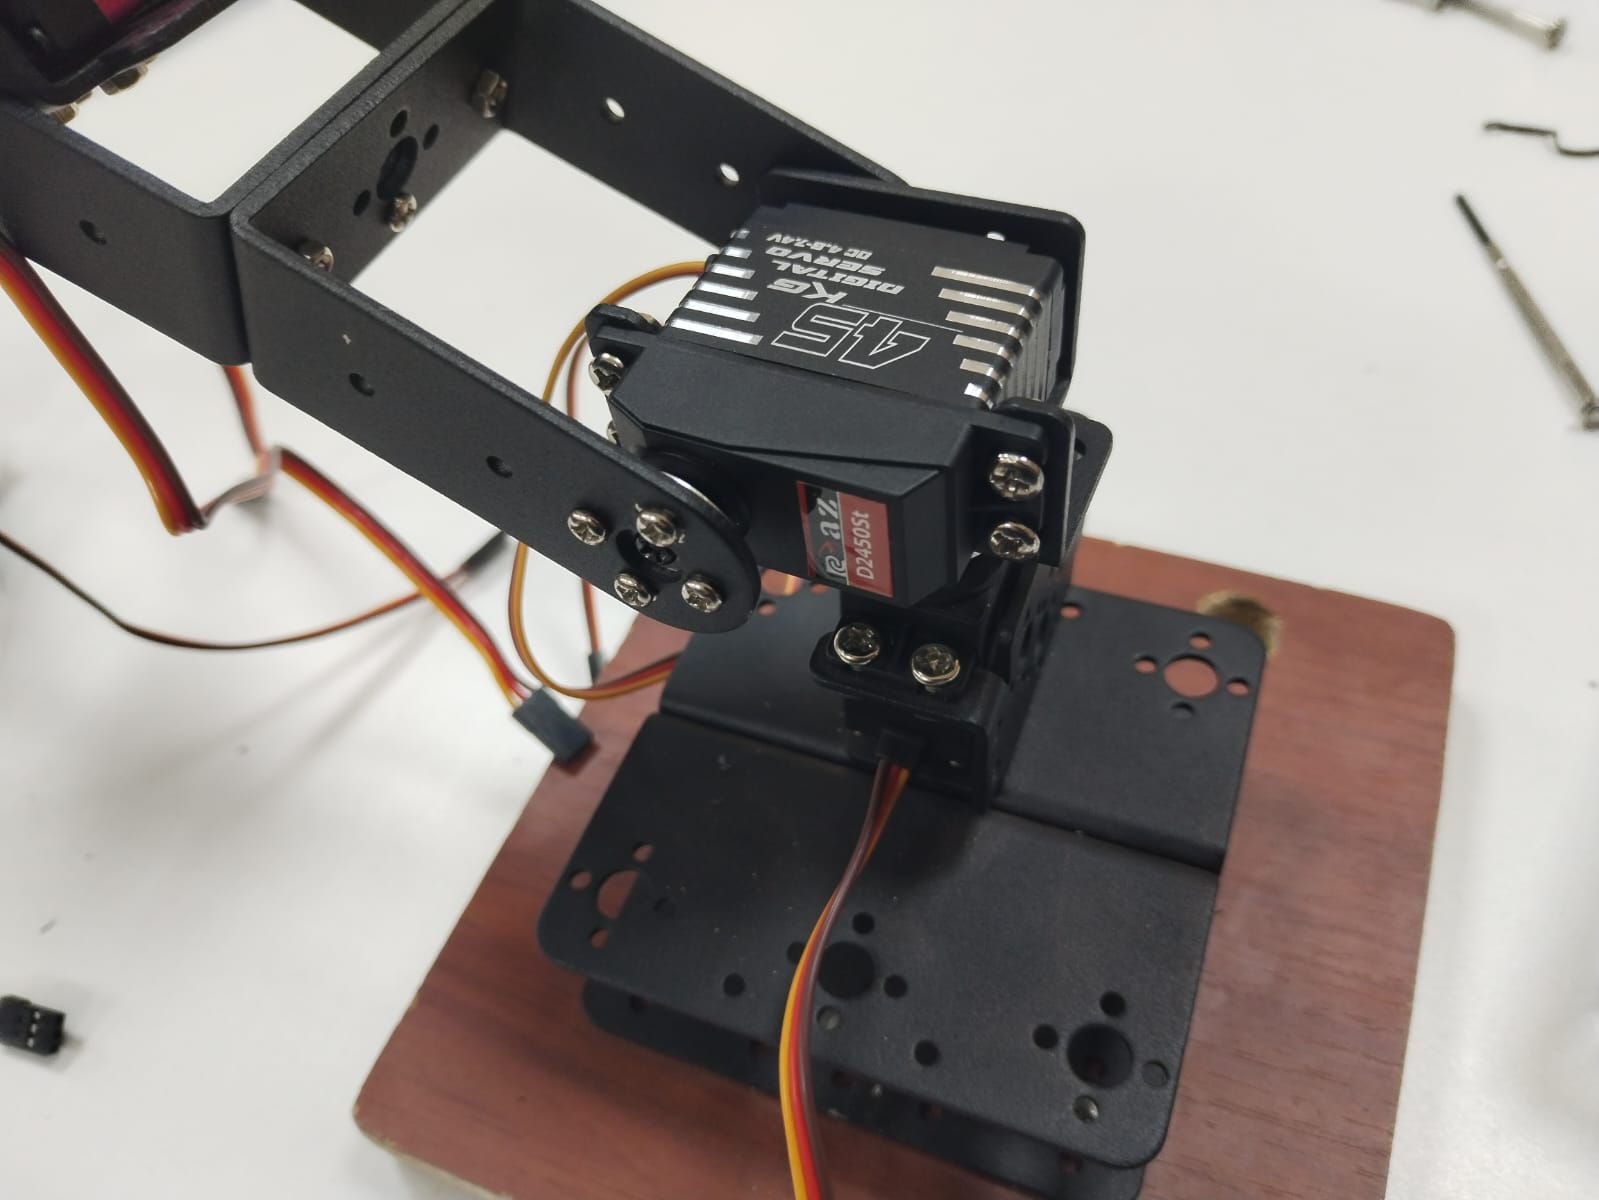
\includegraphics[width=\linewidth, height=4.8cm, keepaspectratio=false]{img/servo_negro_45kg_d2450st.jpeg}
        \caption{Servo 45~kg D2450ST.}
        \label{fig:servo_negro}
    \end{subfigure}
    \hfill
    \begin{subfigure}[b]{0.31\textwidth}
        \centering
        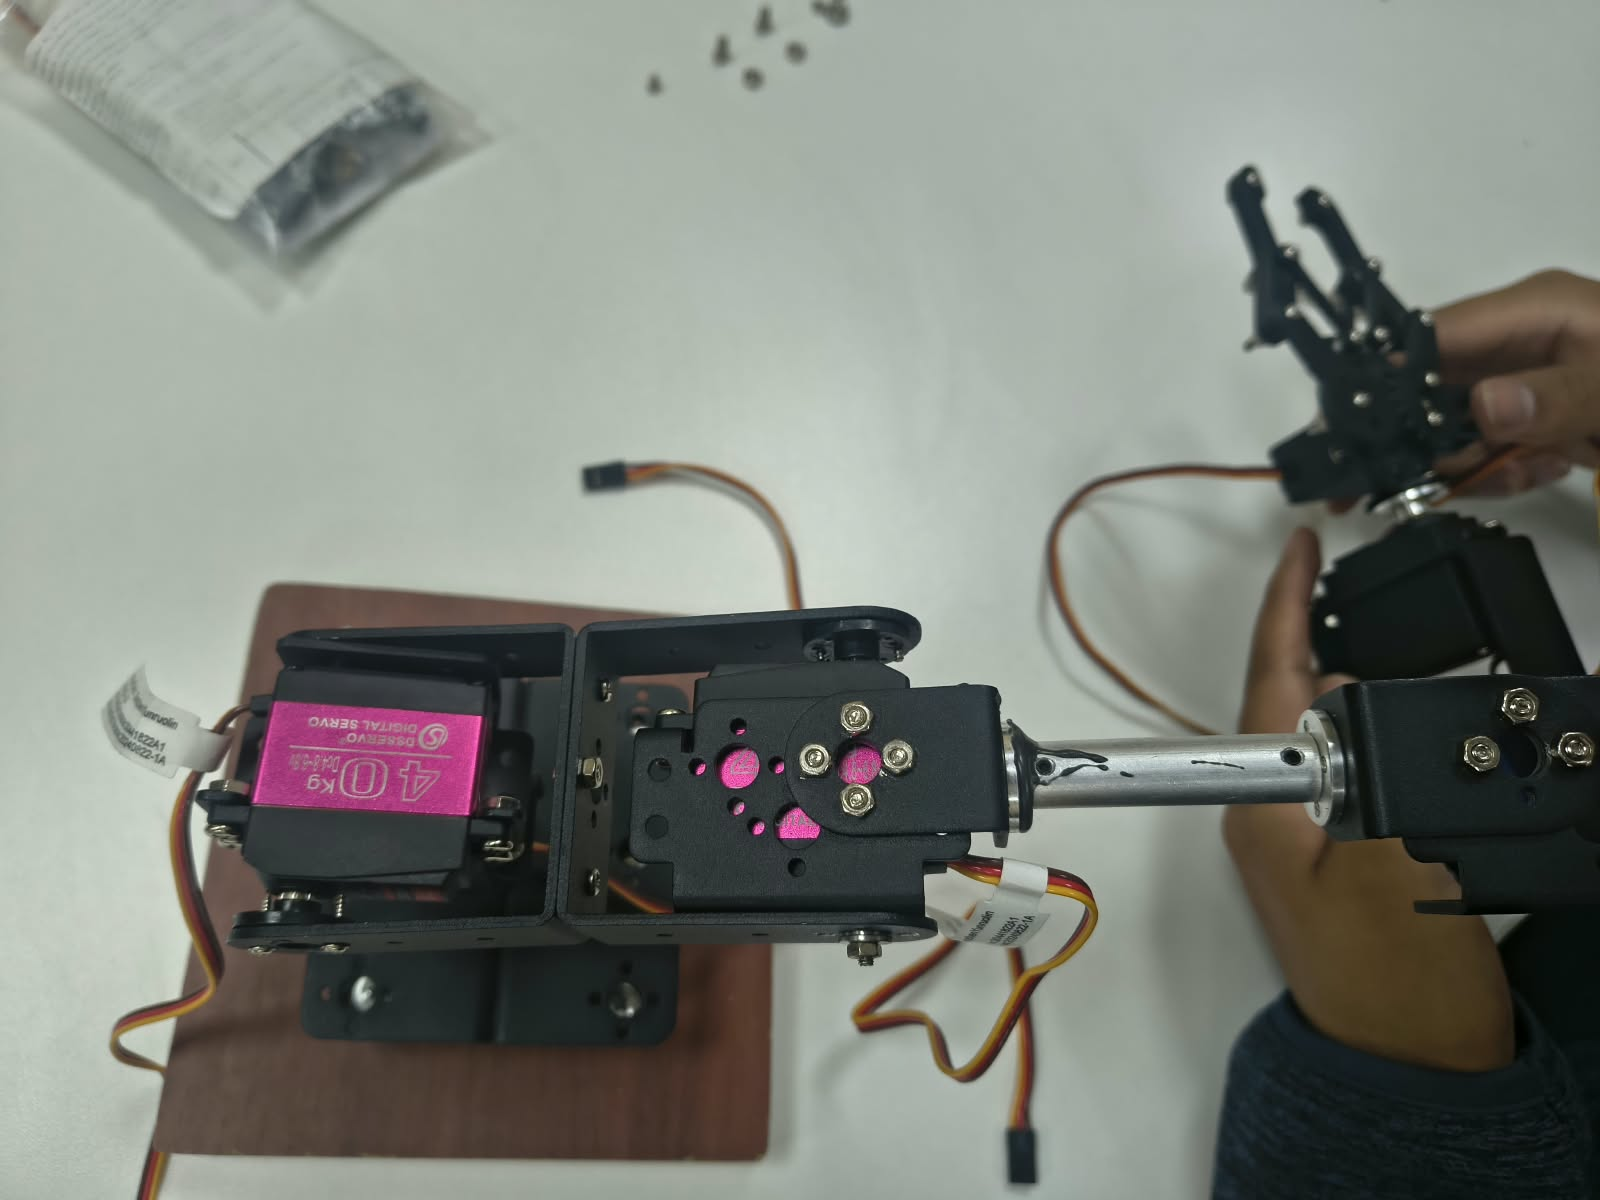
\includegraphics[width=\linewidth, height=4.8cm, keepaspectratio=false]{img/servo_morado_40kg_dsservo.jpeg}
        \caption{Servo 40~kg DSSERVO.}
        \label{fig:servo_morado}
    \end{subfigure}
    \hfill
    \begin{subfigure}[b]{0.31\textwidth}
        \centering
        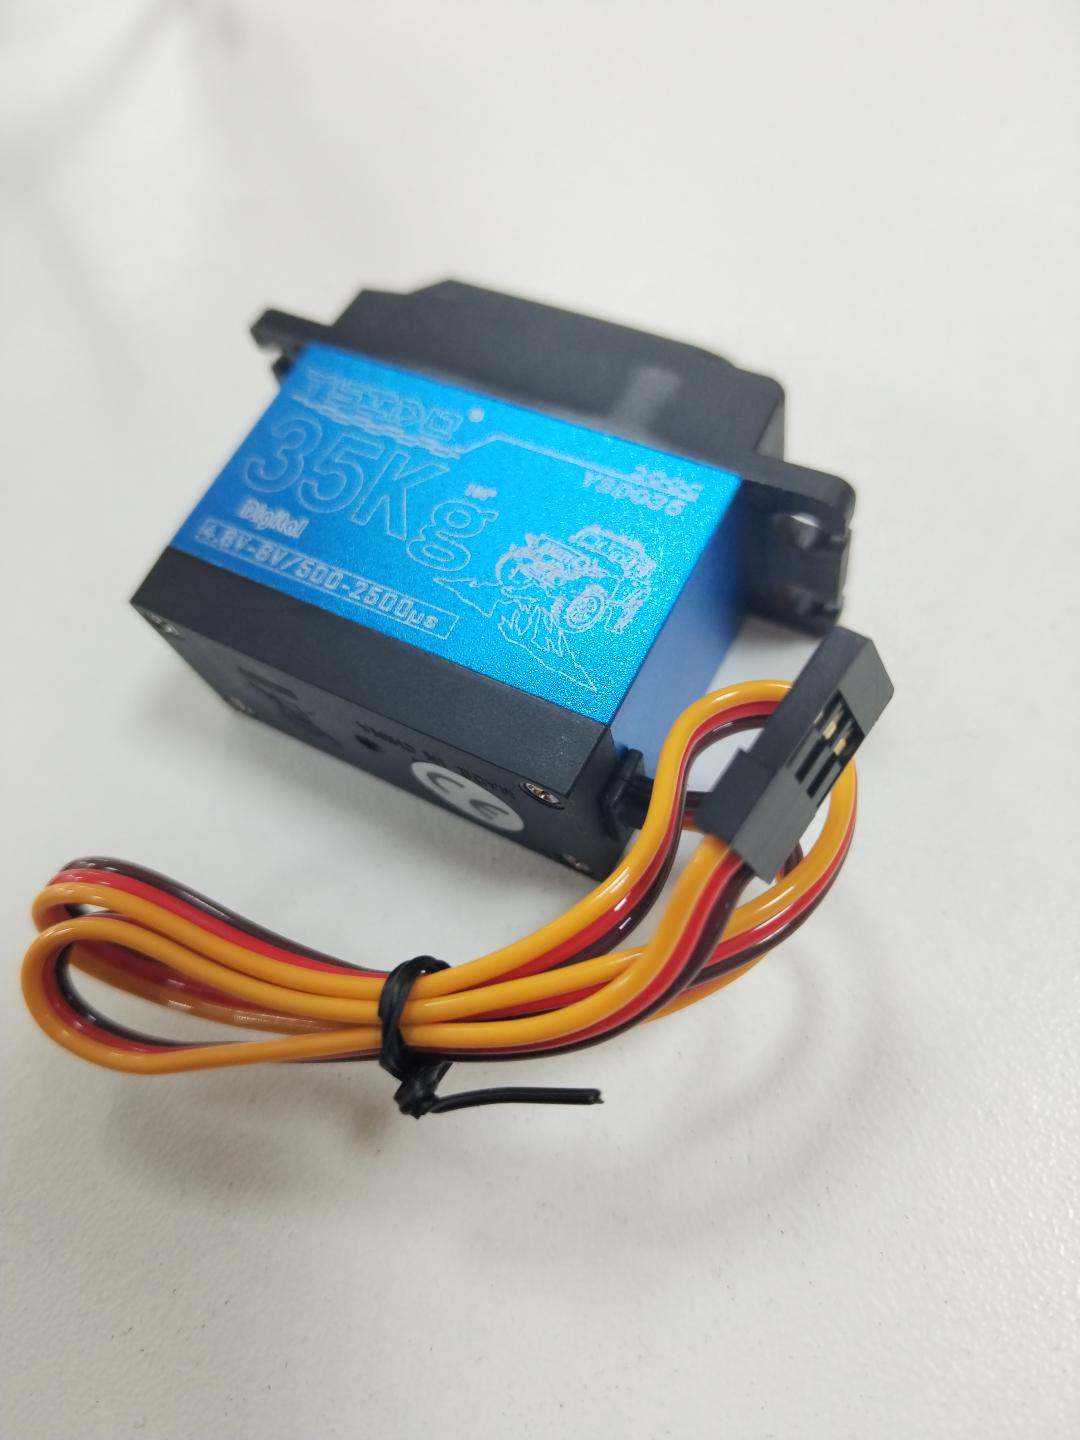
\includegraphics[width=\linewidth, height=4.8cm, keepaspectratio=false]{img/servo_azul_35kg_ysd035.jpeg}
        \caption{Servo 35~kg YSD035.}
        \label{fig:servo_azul}
    \end{subfigure}
    \caption{Actuadores digitales de alta gama inspeccionados para la cadena cinemática.}
    \label{fig:trio_servos}
\end{figure}

% =========================================================
% SECCIÓN 4
% =========================================================
\section{Ensamble Mecánico e Incidencia de Rigidez Articular}

\subsection{Estructuración Física y Base Amortiguadora}
El ensamble del chasis se efectuó empleando perfiles de aleación de aluminio anodizado negro y tornillería métrica M3. Para garantizar la inercia basal y evitar desplazamientos parásitos por el centro de masa dinámico, la estructura completa se apernó a una plataforma de madera aglomerada de alta densidad (Figura~\ref{fig:ensamble_brazo_6gdl}).

\begin{figure}[H]
    \centering
    \begin{subfigure}[b]{0.48\textwidth}
        \centering
        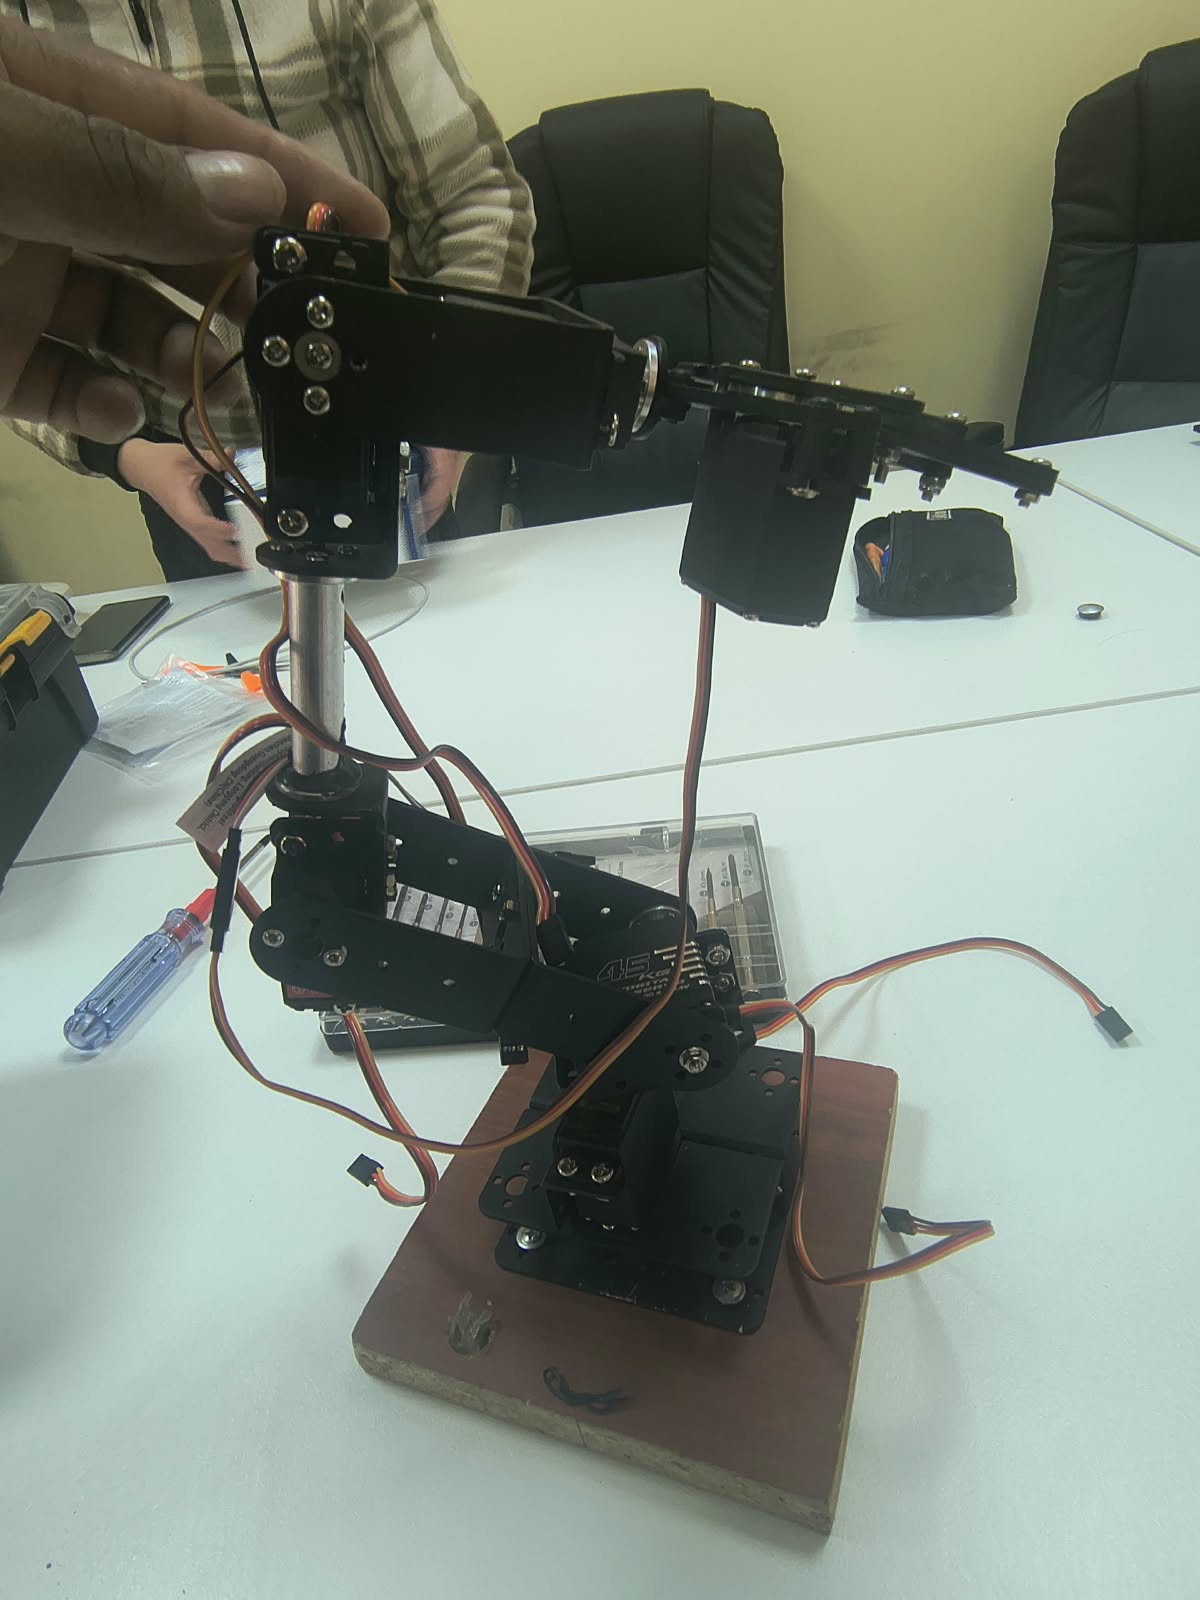
\includegraphics[width=\linewidth, height=6.2cm, keepaspectratio=false]{img/ensamble_general_6gdl.jpeg}
        \caption{Estructura general de 6 GDL erguida.}
        \label{fig:ensamble_6gdl}
    \end{subfigure}
    \hfill
    \begin{subfigure}[b]{0.48\textwidth}
        \centering
        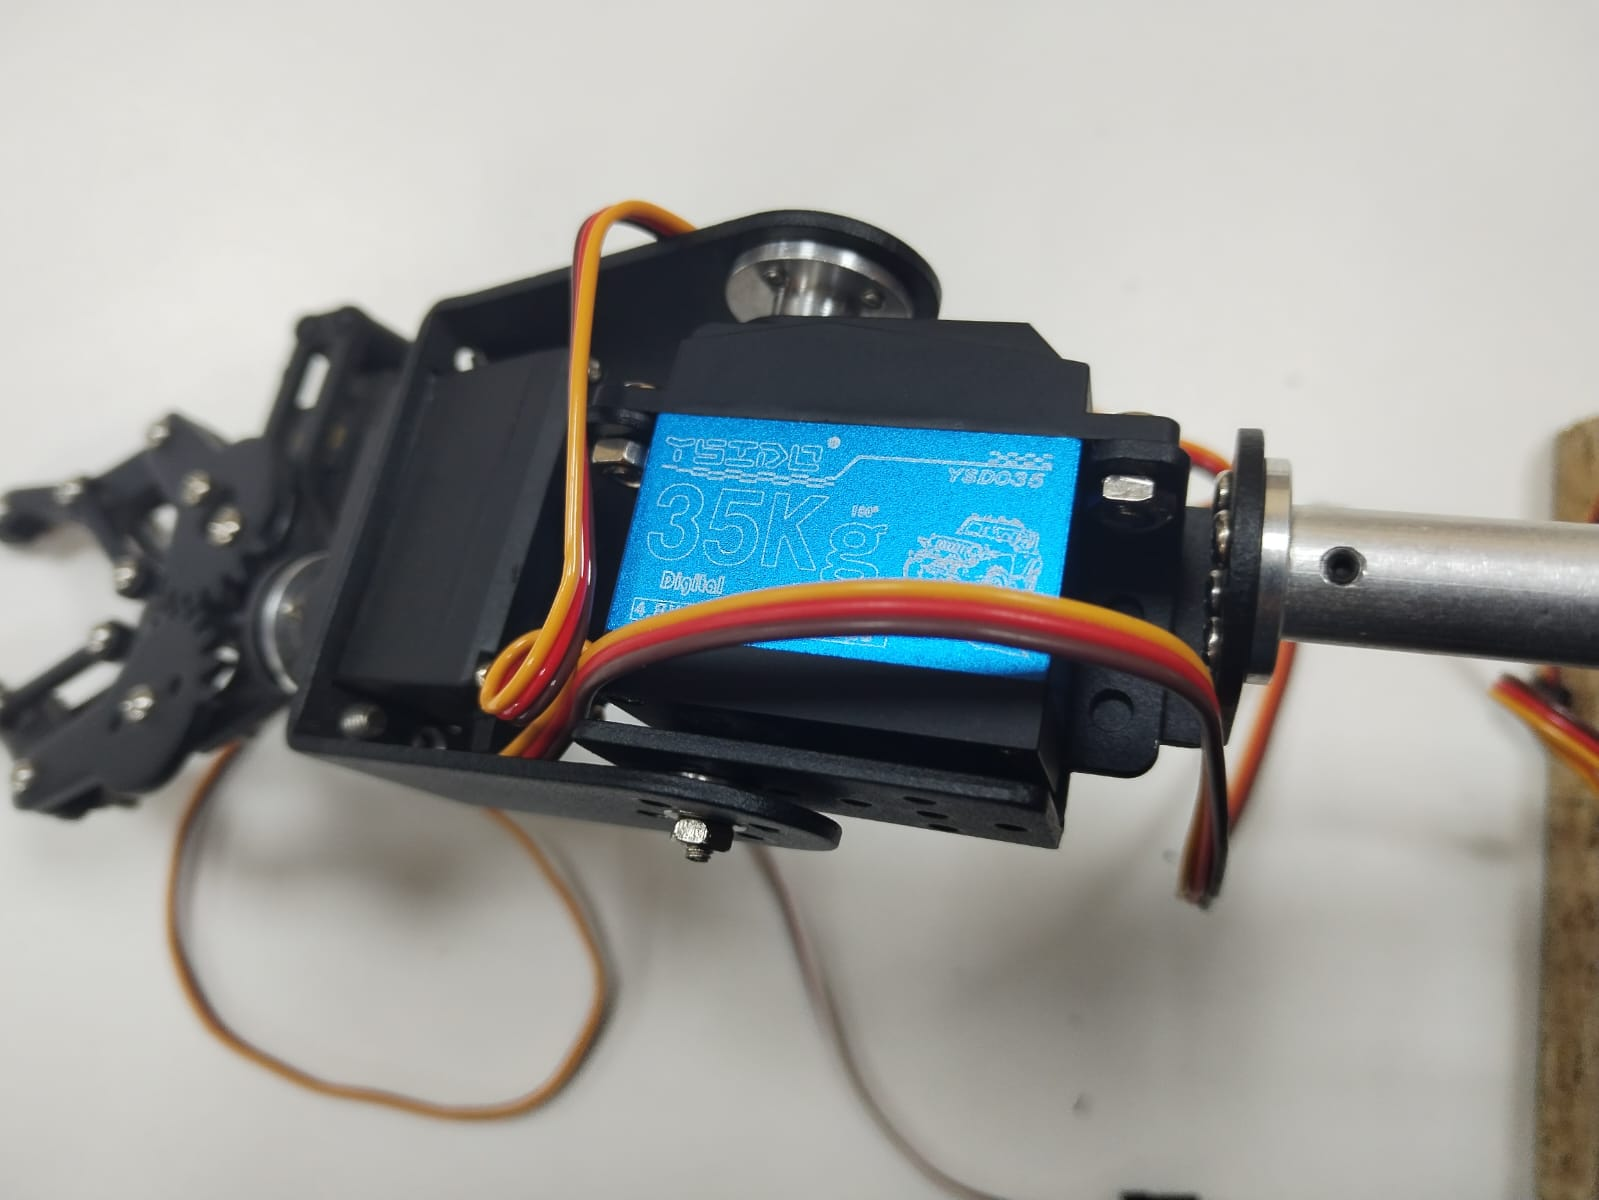
\includegraphics[width=\linewidth, height=6.2cm, keepaspectratio=false]{img/servo_35kg_muneca_eslabon.jpeg}
        \caption{Articulación de muñeca y eslabón cilíndrico.}
        \label{fig:muneca_eslabon}
    \end{subfigure}
    \caption{Montaje de los eslabones mecánicos y articulaciones sobre la base fija.}
    \label{fig:ensamble_brazo_6gdl}
\end{figure}

\subsection{Diagnóstico de la Falla Mecánica: Pérdida de Rigidez en Hombro}

Durante la evaluación de sustentación mecánica en el laboratorio, se presentó un comportamiento anómalo grave: al situar el brazo en posición erguida, la articulación del hombro accionada por el servomotor negro de 45~kg (D2450ST) se mostró completamente suave y sin retención, careciendo de rigidez mecánica y causando el colapso y caída del manipulador hacia adelante bajo la sola acción de la gravedad (Figura~\ref{fig:caida_brazo}).

\begin{figure}[H]
    \centering
    \begin{subfigure}[b]{0.48\textwidth}
        \centering
        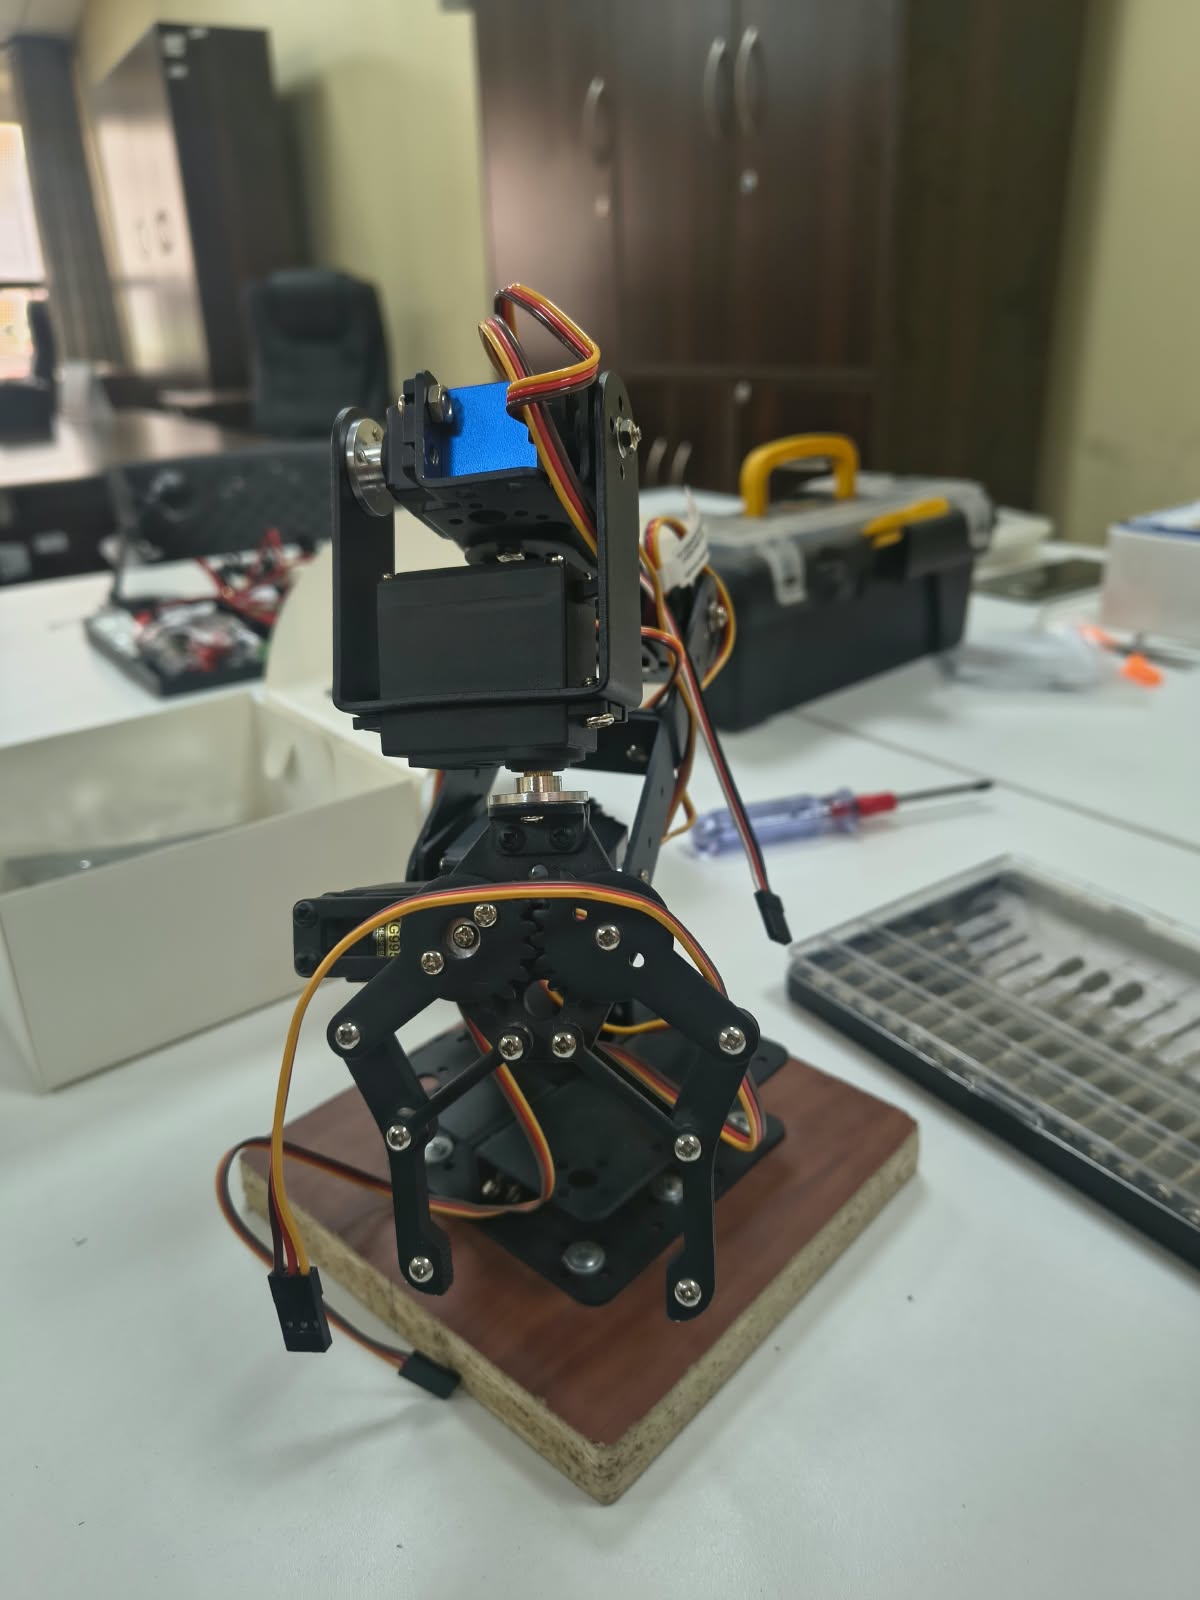
\includegraphics[width=\linewidth, height=6.2cm, keepaspectratio=false]{img/falla_caida_brazo_frontal.jpeg}
        \caption{Caída frontal del brazo sobre la plataforma.}
        \label{fig:caida_frontal}
    \end{subfigure}
    \hfill
    \begin{subfigure}[b]{0.48\textwidth}
        \centering
        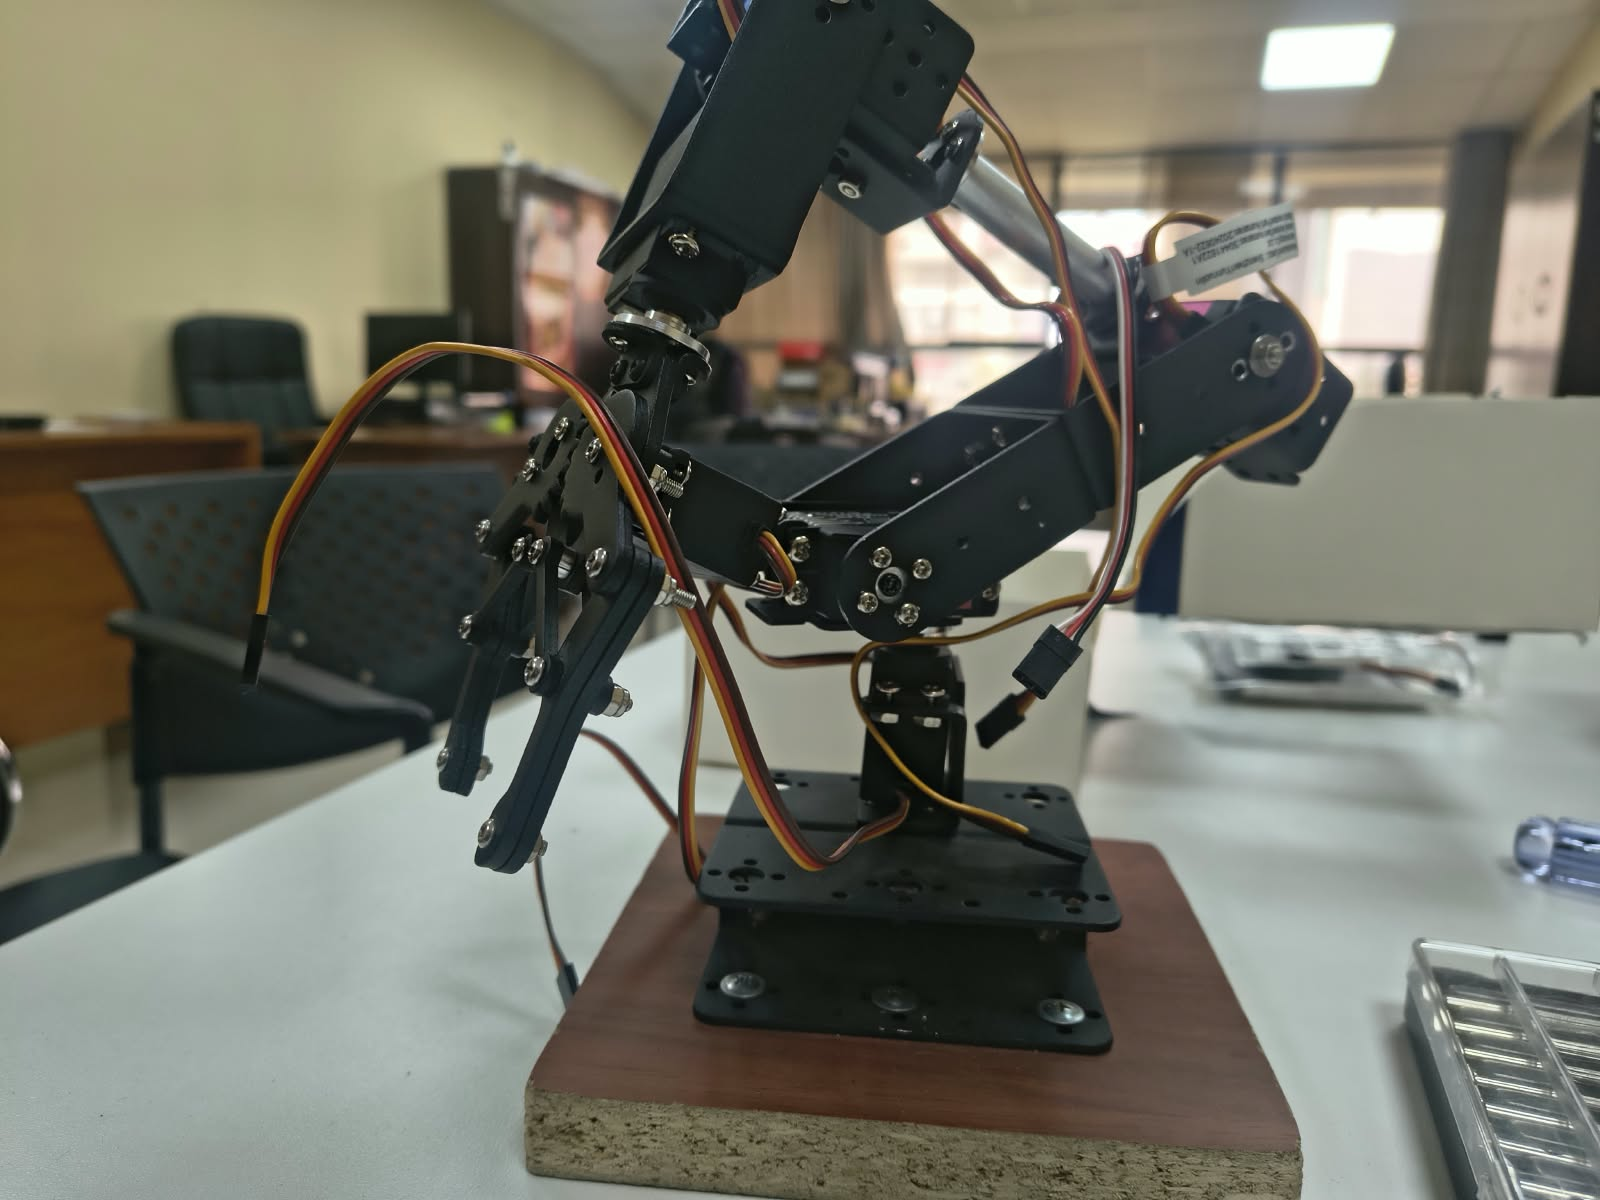
\includegraphics[width=\linewidth, height=6.2cm, keepaspectratio=false]{img/falla_caida_brazo_lateral.jpeg}
        \caption{Pérdida de ángulo y flexión libre del eje.}
        \label{fig:caida_lateral}
    \end{subfigure}
    \caption{Manifestación física de la falla: colapso del brazo por ausencia de rigidez en el servomotor de 45~kg.}
    \label{fig:caida_brazo}
\end{figure}

\begin{alertaincidente}[Ausencia del Perno Axial Central en el Servomotor Negro de 45~kg (D2450ST)]
La inspección visual microscópica (Figura~\ref{fig:macro_perno}) reveló que el disco circular de aluminio (servocuerno) fijado al bracket en U del hombro \textbf{carece del tornillo métrico central que lo une axialmente con el eje estriado del servomotor negro de 45~kg (D2450ST)}. 

Al no existir este tornillo central, los dientes estriados del eje del servomotor patinan en vacío dentro del orificio del servocuerno. Por ende, aunque el motor posea un par nominal de $45\text{ kg}\cdot\text{cm}$, este no se transmite mecánicamente al eslabón del hombro, provocando que la unión se sienta sumamente suave y se produzca la caída inevitable del brazo.
\end{alertaincidente}

\begin{figure}[H]
    \centering
    \begin{subfigure}[b]{0.48\textwidth}
        \centering
        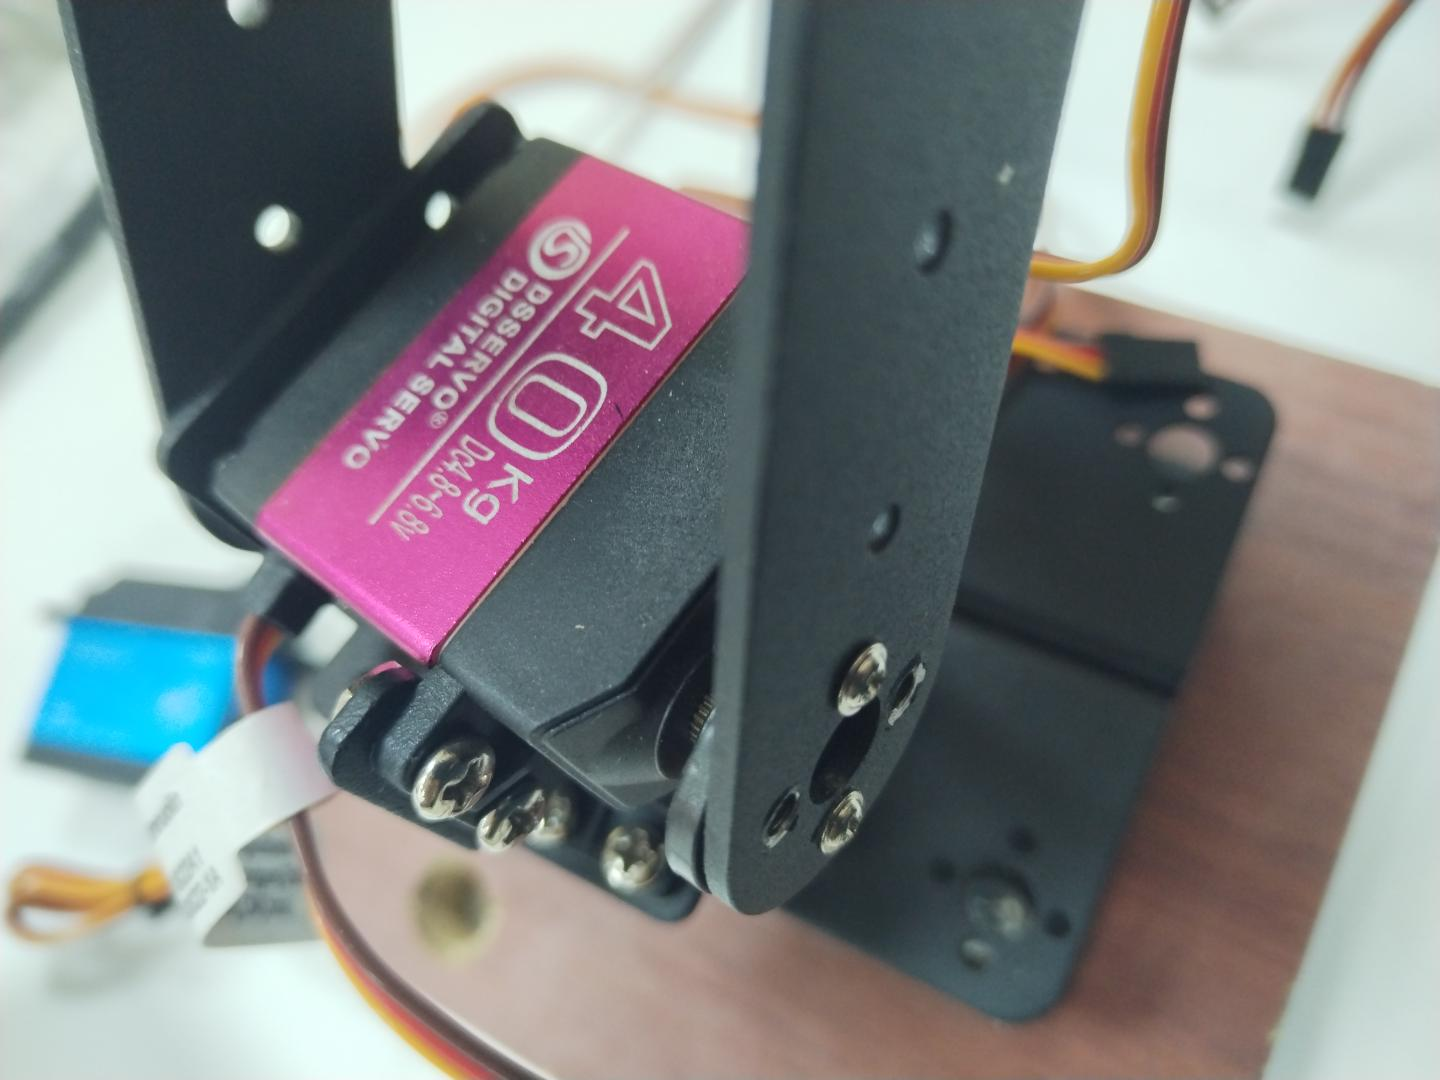
\includegraphics[width=\linewidth, height=5.8cm, keepaspectratio=false]{img/falla_holgura_perno_faltante.jpeg}
        \caption{Macrofotografía: orificio central sin tornillo axial.}
        \label{fig:macro_perno}
    \end{subfigure}
    \hfill
    \begin{subfigure}[b]{0.48\textwidth}
        \centering
        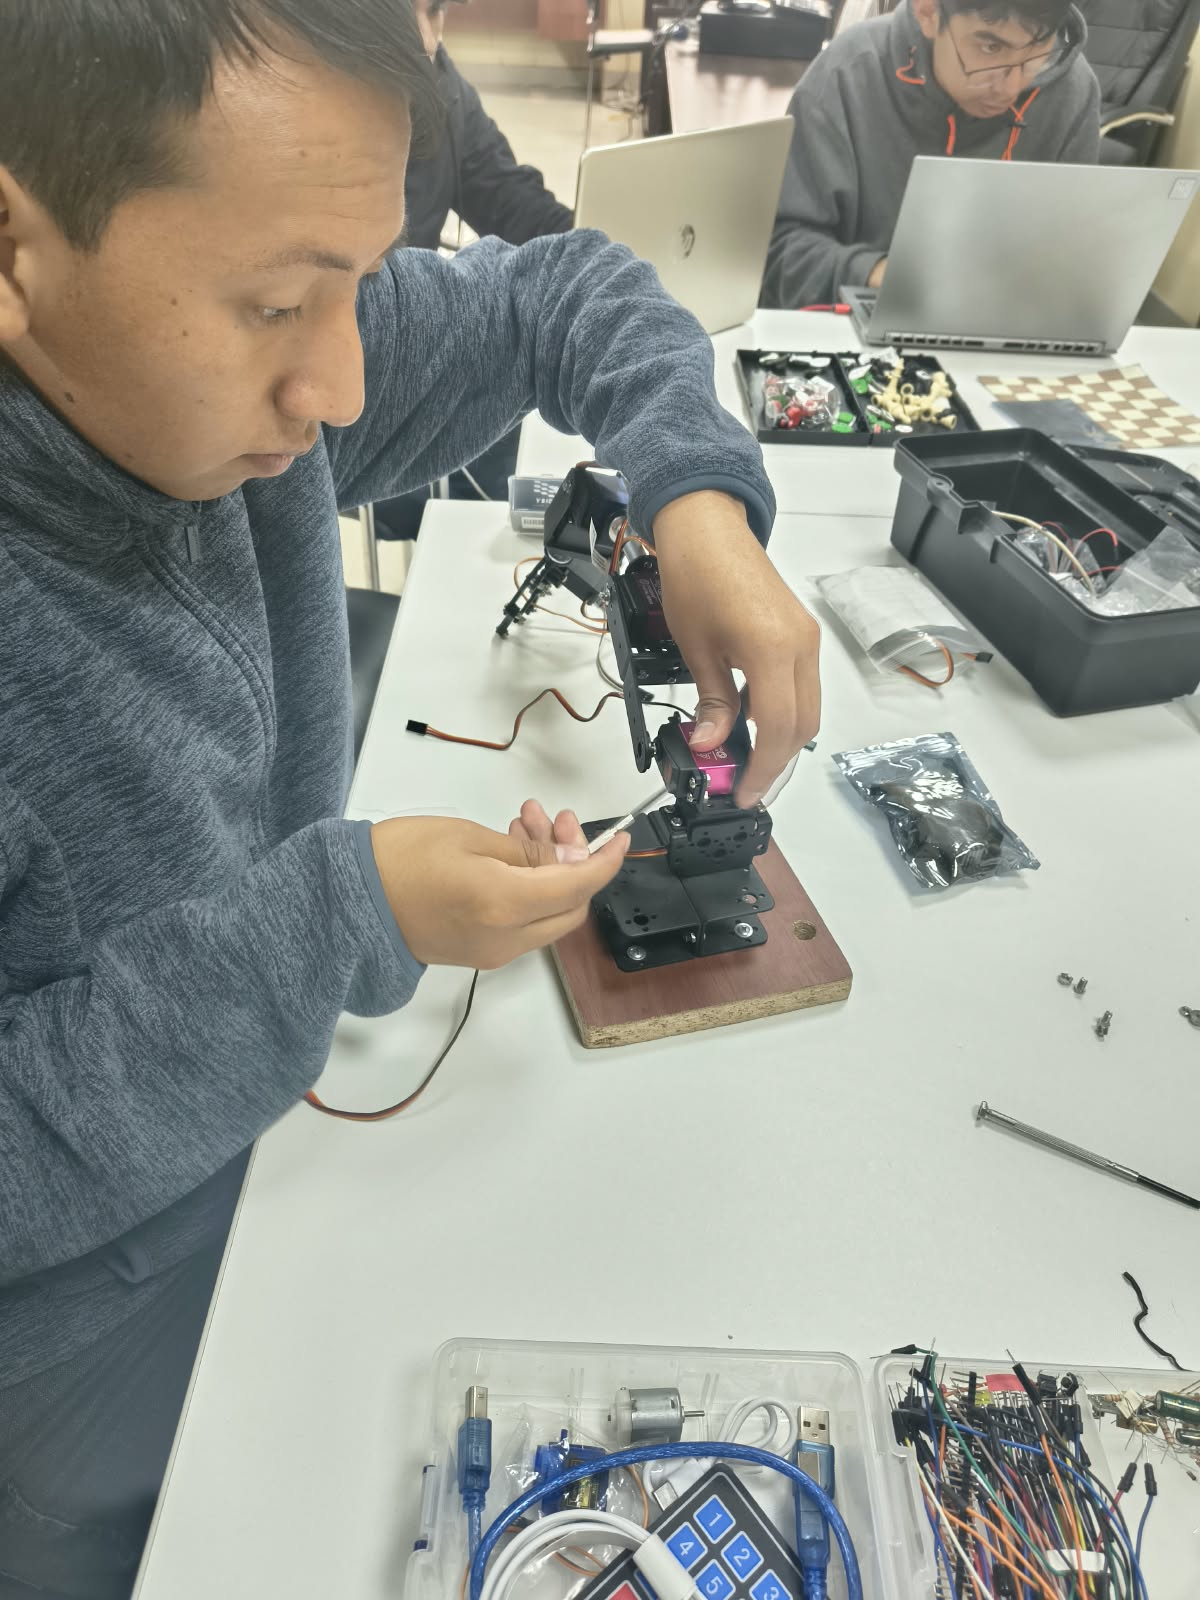
\includegraphics[width=\linewidth, height=5.8cm, keepaspectratio=false]{img/calibracion_mecanica_ajuste.jpeg}
        \caption{Ajuste y alineación con destornillador en UNSAAC.}
        \label{fig:ajuste_herramientas}
    \end{subfigure}
    \caption{Causa raíz identificada y procedimiento de corrección mecánica en banco de trabajo.}
    \label{fig:solucion_mecanica}
\end{figure}

\subsubsection{Plan de Acción y Corrección Inmediata}
Para subsanar definitivamente este fallo previo a la energización:
\begin{enumerate}
    \item Instalar el tornillo axial M3 con arandela de seguridad en el servomotor negro de 45~kg del hombro, así como en los servomotores de codo (40~kg) y muñeca (35~kg).
    \item Aplicar fijador químico de roscas de resistencia media para mitigar desajustes por vibración.
    \item Calibrar mecánicamente la postura de reposo a $90^\circ$ antes de fijar los cuatro pernos perimetrales.
\end{enumerate}

% =========================================================
% SECCIÓN 5
% =========================================================
\section{Diseño Circuital y Plan de Conexionado Eléctrico}

\begin{estadolaboratorio}[Conexión Física Pendiente para la Siguiente Sesión]
Se deja constancia explícita de que, a la fecha del presente informe (v2), **el ESP32-CAM y el módulo PCA9685 aún no han sido interconectados físicamente**. Los componentes se encuentran inspeccionados y los códigos de diagnóstico preparados para su ensamblado eléctrico en la próxima clase.
\end{estadolaboratorio}

\subsection{Topología de Alimentación Desacoplada}
El accionamiento simultáneo de servomotores de 35~kg a 45~kg genera picos de corriente inductiva que superan los 4~A. Con el objetivo de proteger la etapa lógica del ESP32-CAM y prevenir reinicios involuntarios (\textit{brownout}), se diseñó la siguiente arquitectura:
\begin{itemize}
    \item \textbf{Alimentación Lógica (3.3V / 5.0V):} Entregada por el puerto USB de programación hacia el microcontrolador y el pin VCC lógico del PCA9685.
    \item \textbf{Alimentación de Potencia ($V_{ext} = 6.0\text{V}$):} Suministrada por una fuente de alimentación conmutada externa de 6~A hacia la bornera verde de tornillo del PCA9685. El condensador electrolítico integrado de $1000~\mu\text{F}$ suprime los transitorios rápidos.
    \item \textbf{Referencia Común (Star-GND):} Unión en un único punto del pin GND del microcontrolador con el borne GND de potencia del PCA9685 (Figura~\ref{fig:driver_pca}).
\end{itemize}

\begin{figure}[H]
    \centering
    \begin{subfigure}[b]{0.48\textwidth}
        \centering
        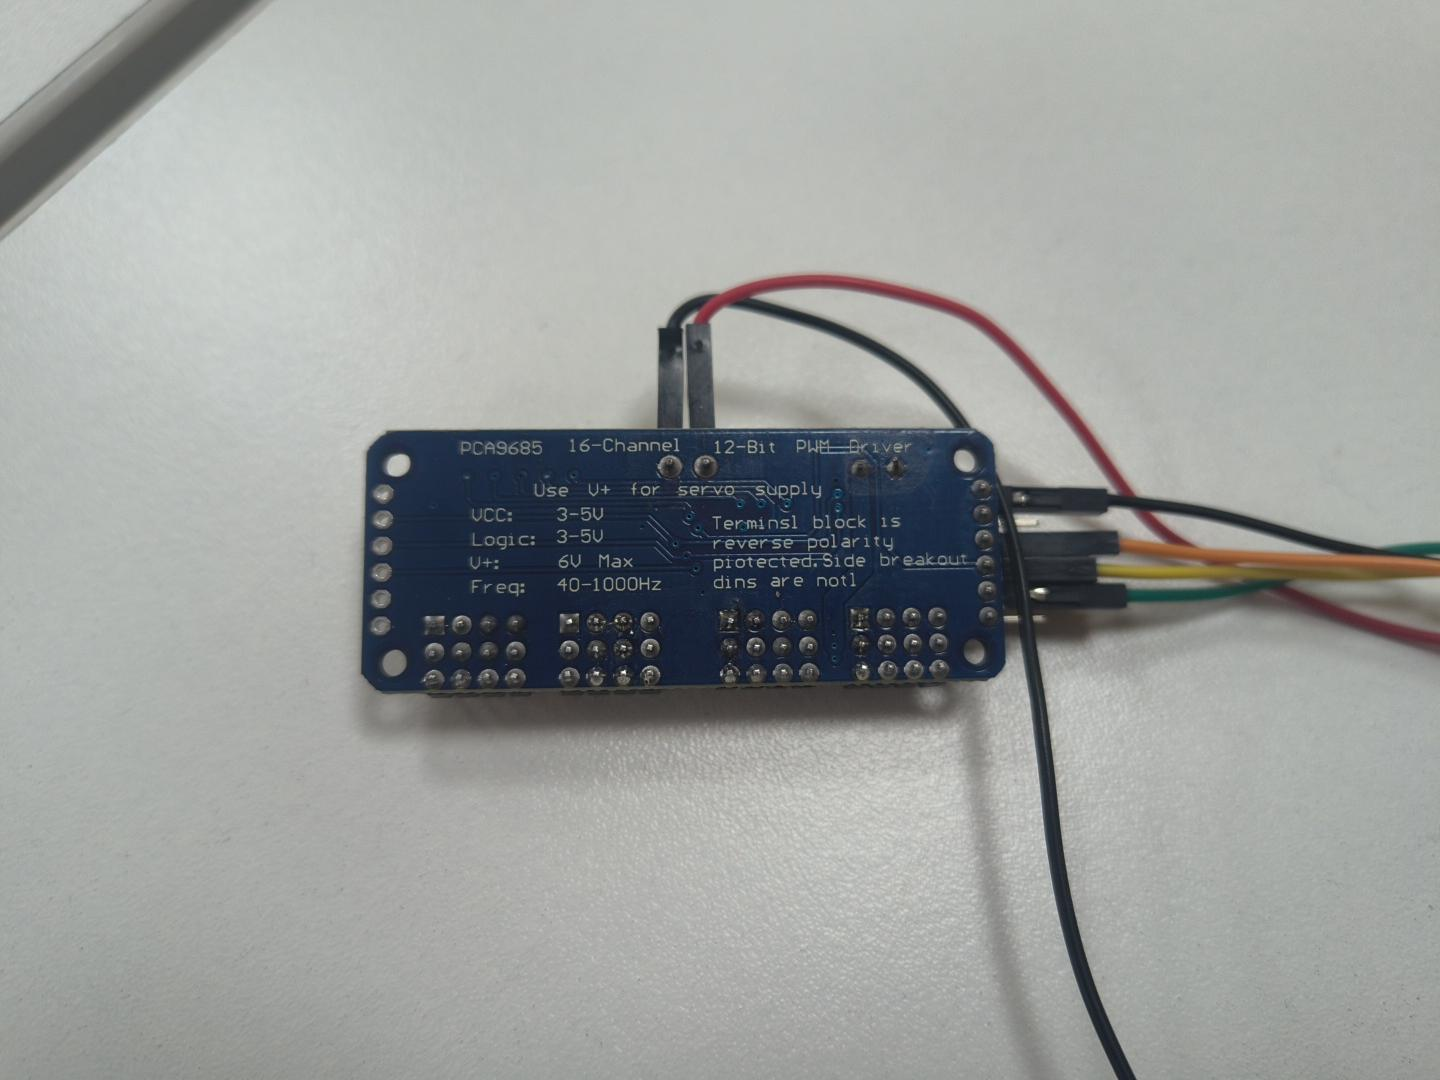
\includegraphics[width=\linewidth, height=5.8cm, keepaspectratio=false]{img/pca9685_pistas_posterior.jpeg}
        \caption{Reverso del PCA9685: límites $V+ \le 6\text{V}$.}
        \label{fig:pca_pistas}
    \end{subfigure}
    \hfill
    \begin{subfigure}[b]{0.48\textwidth}
        \centering
        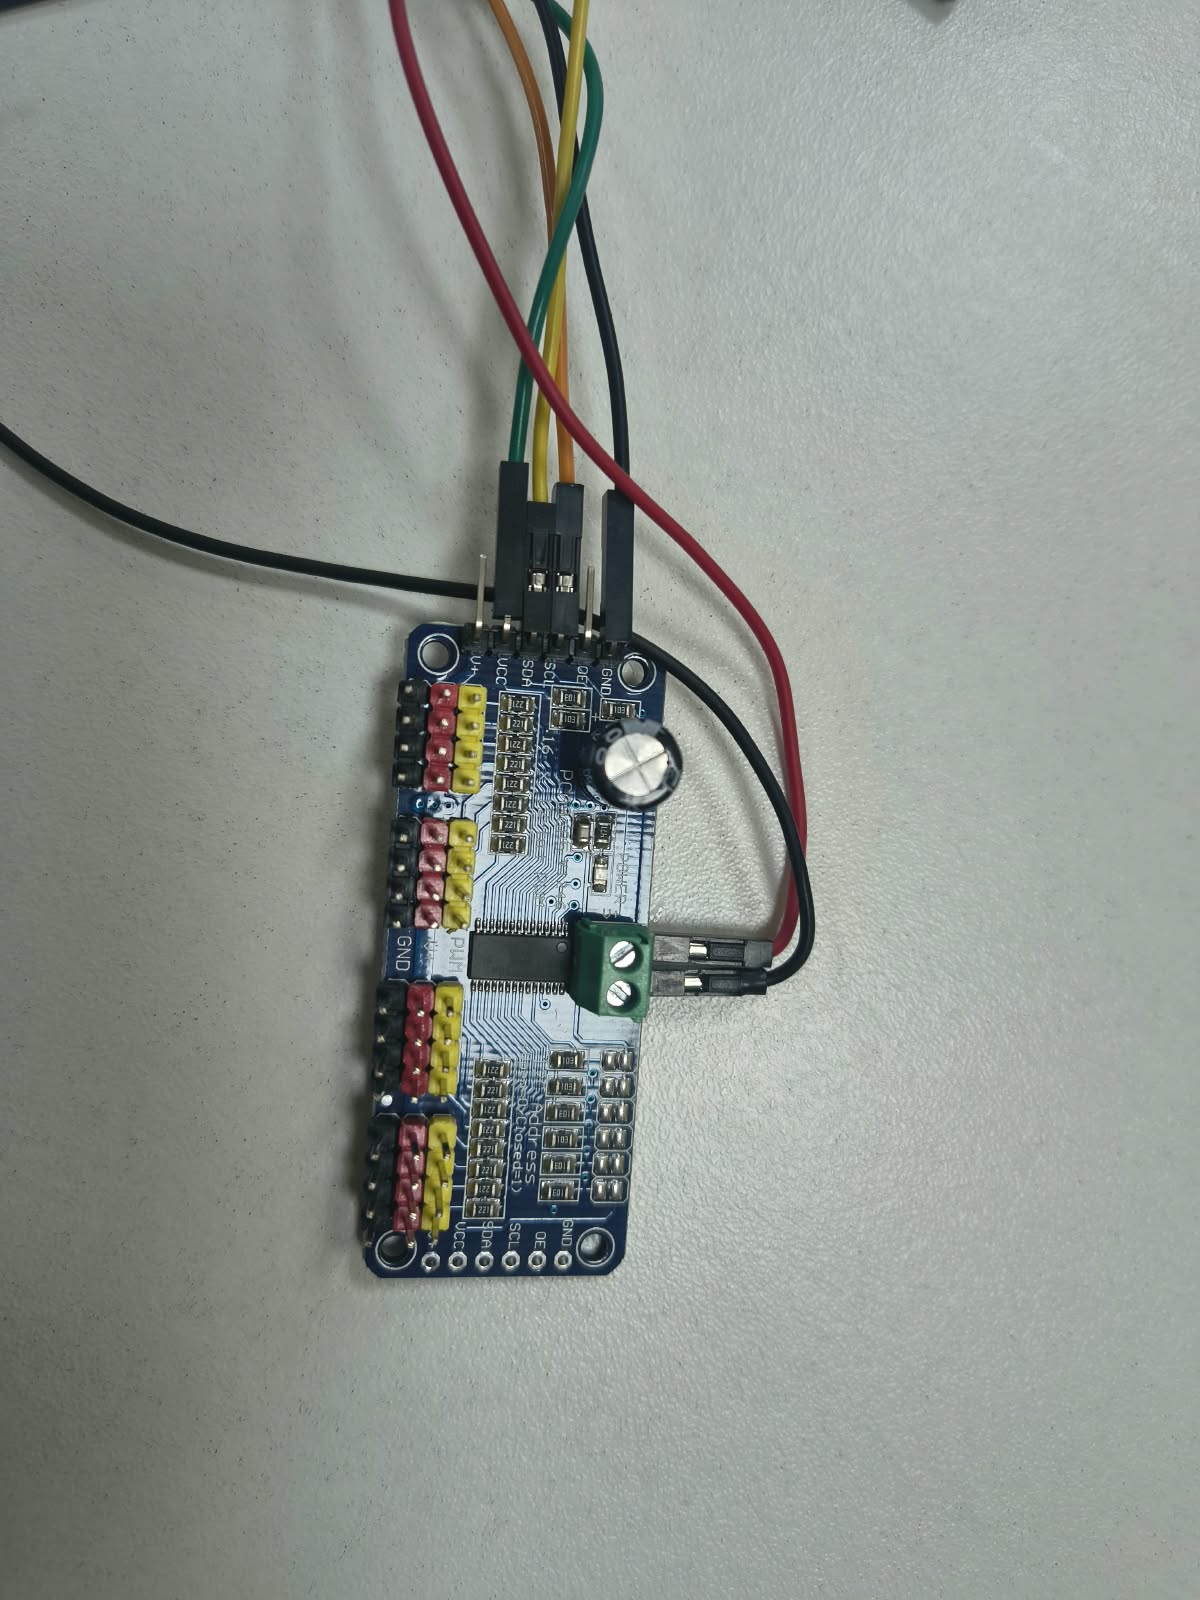
\includegraphics[width=\linewidth, height=5.8cm, keepaspectratio=false]{img/pca9685_conexiones_i2c.jpeg}
        \caption{Líneas I2C y bornera de alta corriente.}
        \label{fig:pca_cables}
    \end{subfigure}
    \caption{Controlador periférico dedicado PCA9685 de 16 canales y 12 bits de resolución.}
    \label{fig:driver_pca}
\end{figure}

\subsection{Asignación de Pines para el Bus \texorpdfstring{$I^2C$}{I2C}}
La interconexión serie entre el procesador y el driver PWM se estableció en terminales seguros que no interfieren con la cámara OV2640:

\begin{table}[H]
\centering
\caption{Tabla Planificada de Conexiones entre ESP32-CAM y PCA9685}
\label{tab:pinout_completo}
\small
\begin{tabularx}{\textwidth}{l l l X}
\toprule
\rowcolor{tableheader}
\textcolor{white}{\textbf{Pin ESP32-CAM}} & \textcolor{white}{\textbf{Pin PCA9685}} & \textcolor{white}{\textbf{Nivel Lógico}} & \textcolor{white}{\textbf{Función y Rol Técnico}} \\
\midrule
GPIO 13 & SDA & 3.3V CMOS & Línea bidireccional de datos del bus $I^2C$ \\
\rowcolor{tablezebra}
GPIO 14 & SCL & 3.3V CMOS & Línea de reloj síncrono del bus $I^2C$ \\
VCC (5V / 3.3V) & VCC & 3.3V / 5.0V & Alimentación del núcleo digital del integrado \\
\rowcolor{tablezebra}
GND & GND & 0V & Masa común digital y de potencia \\
Fuente Ext. (+) & Bornera V+ & 6.0V DC & Riel de potencia exclusivo para servomotores \\
\rowcolor{tablezebra}
Fuente Ext. ($-$) & Bornera GND & 0V & Retorno de corriente de los 6 actuadores \\
\bottomrule
\end{tabularx}
\end{table}

% =========================================================
% SECCIÓN 6
% =========================================================
\section{Arquitectura del Firmware Embebido y Protocolos Web}

El firmware implementado en C++ (\texttt{brazoR.ino}) gestiona concurrentemente la generación de pulsos PWM sobre el PCA9685 y el servicio web HTTP interactivo.

\subsection{Estructuras de Datos y Cinemática Articular}
Cada articulación del robot se modela mediante la estructura \texttt{Joint}, garantizando límites angulares seguros por software para proteger los eslabones metálicos:
\begin{itemize}
    \item \textbf{Canales PWM:} Asignados correlativamente del 0 al 5 en el PCA9685.
    \item \textbf{Rango Seguro:} Acotado estrictamente en $[30^\circ, 150^\circ]$ con posición de reposo (\textit{HOME}) en $90^\circ$.
    \item \textbf{Ancho de Pulsos:} Rango calibrado de 1000~$\mu$s a 2000~$\mu$s (ampliable a 500--2500~$\mu$s según motor).
\end{itemize}

\subsection{Mecanismos de Seguridad: Watchdog de Enlace}
Para prevenir accidentes en caso de que el operador pierda la cobertura Wi-Fi:
\begin{itemize}
    \item \textbf{Temporizador de Heartbeat (\texttt{LINK\_TIMEOUT\_MS = 10000}):} Si transcurren más de 10 segundos sin recibir peticiones HTTP, se dispara automáticamente la rutina \texttt{stopAll()}.
    \item \textbf{Corte de Pulsos (\texttt{stopAll()}):} Escribe el bit \texttt{FULL\_OFF} mediante \texttt{pwm.setPWM(ch, 0, 4096)}, suspendiendo la modulación para evitar sobrecalentamiento en los motores.
\end{itemize}

\subsection{Servidor Web Autónomo y API REST}
El ESP32-CAM inicializa un Punto de Acceso (\textit{SoftAP}) con SSID \texttt{Brazo-ESP32CAM} en la dirección IP \texttt{192.168.4.1}. La página web se aloja comprimida en memoria de programa (\texttt{PROGMEM}) en \texttt{pagina.h}, consumiendo los siguientes endpoints REST:
\begin{itemize}
    \item \texttt{GET /api/status}: Telemetría completa de ángulos y estados en formato JSON.
    \item \texttt{POST /api/servo}: Actualiza el ángulo objetivo de una articulación específica.
    \item \texttt{POST /api/enable}: Activa o desactiva individualmente el pulso de un servo.
    \item \texttt{POST /api/home}: Envía los servos activos a su postura central de $90^\circ$.
    \item \texttt{POST /api/stop}: Parada de emergencia instantánea en todos los canales.
\end{itemize}

\newpage

% =========================================================
% SECCIÓN 7
% =========================================================
\section{Código Fuente Completo del Firmware}

A continuación se transcribe el código fuente completo del firmware desarrollado para el microcontrolador ESP32-CAM (\texttt{codigo/firmware\_brazo\_esp32/brazoR.ino}):

\begin{lstlisting}[language=C++, caption={Firmware completo del brazo robótico (brazoR.ino)}]
#include <Arduino.h>
#include <Wire.h>
#include <WiFi.h>
#include <WebServer.h>
#include <Adafruit_PWMServoDriver.h>

#undef HTTP_ANY
#include "camara.h"
#include "pagina.h"

// Credenciales del Punto de Acceso (SoftAP)
constexpr char AP_NAME[] = "Brazo-ESP32CAM";
constexpr char AP_PASSWORD[] = "CambiaEstaClave123";
constexpr uint8_t SDA_PIN = 13;
constexpr uint8_t SCL_PIN = 14;
constexpr uint8_t PCA_ADDRESS = 0x40;
constexpr uint32_t LINK_TIMEOUT_MS = 10000;
constexpr uint32_t MOTION_INTERVAL_MS = 20;

struct Joint {
  const char *name;
  uint8_t channel;
  uint8_t minAngle;
  uint8_t maxAngle;
  uint8_t home;
  uint16_t minPulseUs;
  uint16_t maxPulseUs;
  uint8_t current;
  uint8_t target;
  bool enabled;
};

// Limites seguros de operacion: calibrar previo a montaje definitivo
Joint joints[] = {
    {"Base",       0, 30, 150, 90, 1000, 2000, 90, 90, false},
    {"Hombro",     1, 30, 150, 90, 1000, 2000, 90, 90, false},
    {"Codo",       2, 30, 150, 90, 1000, 2000, 90, 90, false},
    {"Muneca 1",   3, 30, 150, 90, 1000, 2000, 90, 90, false},
    {"Muneca 2",   4, 30, 150, 90, 1000, 2000, 90, 90, false},
    {"Pinza",      5, 30, 150, 90, 1000, 2000, 90, 90, false},
};
constexpr size_t JOINT_COUNT = sizeof(joints) / sizeof(joints[0]);

Adafruit_PWMServoDriver pwm(PCA_ADDRESS, Wire);
WebServer server(80);
bool driverReady = false;
uint32_t lastHeartbeat = 0;
uint32_t lastMotion = 0;

bool parseNumber(const String &value, int &out) {
  if (value.isEmpty() || value.length() > 3) return false;
  int number = 0;
  for (size_t i = 0; i < value.length(); ++i) {
    if (value[i] < '0' || value[i] > '9') return false;
    number = number * 10 + (value[i] - '0');
  }
  out = number;
  return true;
}

void json(int code, const String &body) {
  server.sendHeader("Cache-Control", "no-store");
  server.sendHeader("X-Content-Type-Options", "nosniff");
  server.send(code, "application/json; charset=utf-8", body);
}

void stopAll() {
  if (!driverReady) return;
  for (Joint &joint : joints) {
    pwm.setPWM(joint.channel, 0, 4096); // FULL_OFF
    joint.enabled = false;
    joint.target = joint.current;
  }
}

void writeAngle(Joint &joint) {
  const uint16_t pulse = map(joint.current, 0, 180,
                             joint.minPulseUs, joint.maxPulseUs);
  pwm.writeMicroseconds(joint.channel, pulse);
}

bool selectedJoint(Joint *&joint) {
  int index;
  if (!server.hasArg("i") || !parseNumber(server.arg("i"), index) ||
      index >= static_cast<int>(JOINT_COUNT)) {
    json(400, "{\"error\":\"Indice de servo invalido\"}");
    return false;
  }
  joint = &joints[index];
  return true;
}

bool requireDriver() {
  if (!driverReady) {
    json(503, "{\"error\":\"PCA9685 no detectado: revisar conexion I2C\"}");
    return false;
  }
  return true;
}

void sendStatus() {
  String body;
  body.reserve(780);
  body = "{\"ready\":";
  body += driverReady ? "true" : "false";
  body += ",\"camera\":";
  body += cameraReady ? "true" : "false";
  body += ",\"psram\":";
  body += psramReady ? "true" : "false";
  body += ",\"servos\":[";
  for (size_t i = 0; i < JOINT_COUNT; ++i) {
    const Joint &joint = joints[i];
    if (i) body += ',';
    body += "{\"name\":\"";
    body += joint.name;
    body += "\",\"angle\":";
    body += String(joint.current);
    body += ",\"target\":";
    body += String(joint.target);
    body += ",\"min\":";
    body += String(joint.minAngle);
    body += ",\"max\":";
    body += String(joint.maxAngle);
    body += ",\"enabled\":";
    body += joint.enabled ? "true" : "false";
    body += '}';
  }
  body += "]}";
  json(200, body);
}

void enableJoint() {
  if (!requireDriver()) return;
  Joint *joint;
  if (!selectedJoint(joint)) return;
  int on;
  if (!server.hasArg("on") || !parseNumber(server.arg("on"), on) || on > 1) {
    json(400, "{\"error\":\"on debe ser 0 o 1\"}");
    return;
  }
  if (on) {
    if (!joint->enabled) {
      joint->current = joint->home;
      joint->target = joint->home;
      writeAngle(*joint);
      joint->enabled = true;
    }
    lastHeartbeat = millis();
  } else {
    pwm.setPWM(joint->channel, 0, 4096);
    joint->enabled = false;
    joint->target = joint->current;
  }
  sendStatus();
}

void setAngle() {
  if (!requireDriver()) return;
  Joint *joint;
  if (!selectedJoint(joint)) return;
  int angle;
  if (!server.hasArg("angle") || !parseNumber(server.arg("angle"), angle) ||
      angle < joint->minAngle || angle > joint->maxAngle) {
    json(400, "{\"error\":\"Angulo fuera de los limites configurados\"}");
    return;
  }
  if (!joint->enabled) {
    json(409, "{\"error\":\"Activar primero este servo\"}");
    return;
  }
  joint->target = angle;
  lastHeartbeat = millis();
  sendStatus();
}

void home() {
  if (!requireDriver()) return;
  for (Joint &joint : joints) {
    if (joint.enabled) joint.target = joint.home;
  }
  lastHeartbeat = millis();
  sendStatus();
}

void moveServos() {
  const uint32_t now = millis();
  bool anyEnabled = false;
  for (const Joint &joint : joints) anyEnabled |= joint.enabled;
  if (anyEnabled && now - lastHeartbeat >= LINK_TIMEOUT_MS) {
    stopAll();
    Serial.println("Sin latido del navegador: PWM desactivado");
  }
  if (now - lastMotion < MOTION_INTERVAL_MS) return;
  lastMotion = now;
  for (Joint &joint : joints) {
    if (!joint.enabled || joint.current == joint.target) continue;
    joint.current += (joint.current < joint.target) ? 1 : -1;
    writeAngle(joint);
  }
}

void setup() {
  Serial.begin(115200);
  startCamera();
  Wire.begin(SDA_PIN, SCL_PIN);
  Wire.setClock(100000);
  driverReady = pwm.begin();
  if (driverReady) {
    pwm.setPWMFreq(50);
    stopAll();
  } else {
    Serial.println("PCA9685 no detectado en 0x40. Revisar SDA/SCL, GND y VCC.");
  }

  WiFi.mode(WIFI_AP);
  WiFi.softAPConfig(IPAddress(192, 168, 4, 1), IPAddress(192, 168, 4, 1),
                    IPAddress(255, 255, 255, 0));
  if (!WiFi.softAP(AP_NAME, AP_PASSWORD)) {
    Serial.println("ERROR: no se pudo crear la red Wi-Fi");
    return;
  }
  server.on("/", HTTP_GET, []() {
    server.sendHeader("Cache-Control", "no-store");
    server.send_P(200, "text/html; charset=utf-8", INDEX_HTML);
  });
  server.on("/api/status", HTTP_GET, sendStatus);
  server.on("/api/enable", HTTP_POST, enableJoint);
  server.on("/api/servo", HTTP_POST, setAngle);
  server.on("/api/home", HTTP_POST, home);
  server.on("/api/stop", HTTP_POST, []() { stopAll(); sendStatus(); });
  server.on("/api/heartbeat", HTTP_POST, []() {
    lastHeartbeat = millis();
    sendStatus();
  });
  server.onNotFound([]() { json(404, "{\"error\":\"Ruta no encontrada\"}"); });
  server.begin();
  startCameraStream();
  Serial.print("Conectar a ");
  Serial.print(AP_NAME);
  Serial.print("; abrir http://");
  Serial.println(WiFi.softAPIP());
}

void loop() {
  server.handleClient();
  moveServos();
}
\end{lstlisting}

\newpage

% =========================================================
% SECCIÓN 8
% =========================================================
\section{Pruebas Experimentales y Hoja de Ruta (Versión 2)}

Durante la jornada de trabajo desarrollada en el laboratorio de robótica (Figura~\ref{fig:estudiantes_trabajo}), los estudiantes completaron el análisis físico del prototipo y el dimensionamiento de las etapas de potencia.

\begin{figure}[H]
    \centering
    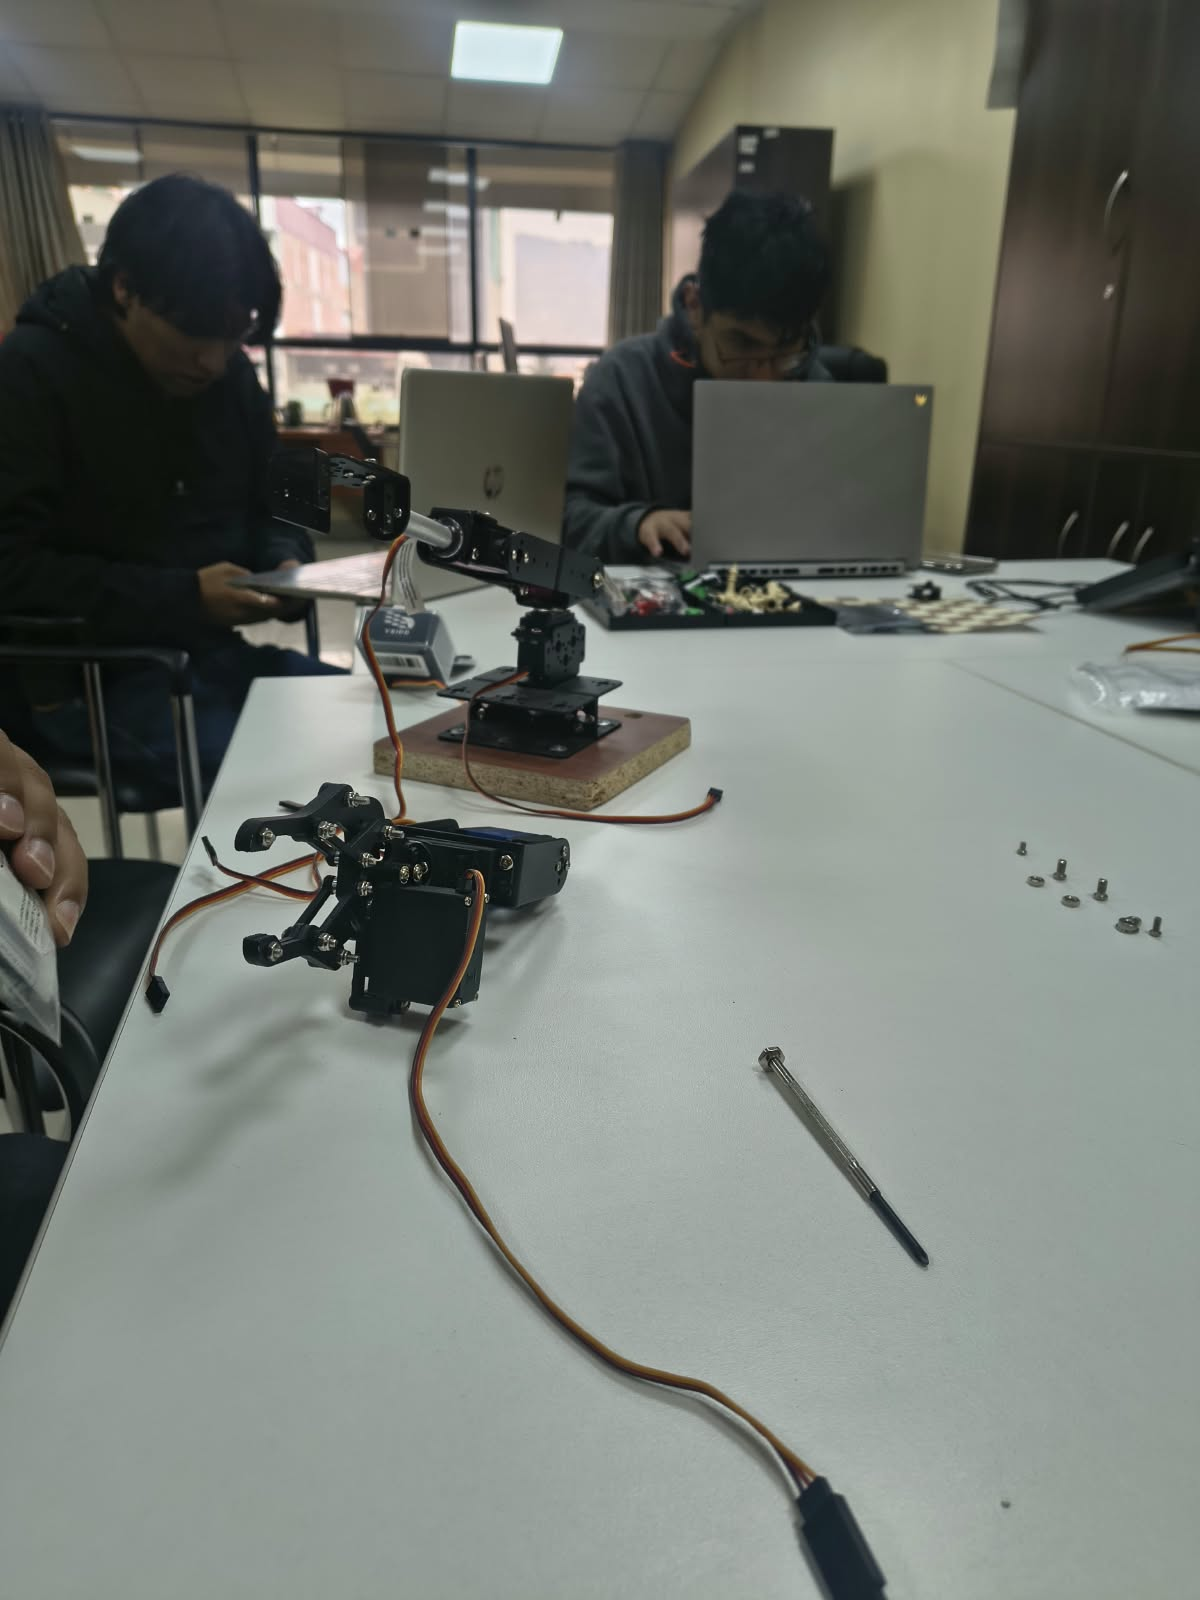
\includegraphics[width=0.72\textwidth, height=7.5cm, keepaspectratio=false]{img/estudiantes_laboratorio_desarrollo.jpeg}
    \caption{Equipo de estudiantes durante la sesión de ensamblado y diagnóstico en laboratorio UNSAAC.}
    \label{fig:estudiantes_trabajo}
\end{figure}

\subsection{Cronograma de Integración Física para la Versión 2}
En la siguiente sesión de laboratorio se ejecutará la secuencia de puesta en marcha definitiva:
\begin{enumerate}
    \item \textbf{Corrección Mecánica de Articulaciones:} Colocación de los tornillos axiales M3 en los servocuernos de aluminio (priorizando el servomotor negro de 45~kg del hombro) para asegurar la transmisión rígida de par y eliminar el juego articular.
    \item \textbf{Verificación del Bus \texorpdfstring{$I^2C$}{I2C}:} Carga del programa de diagnóstico \texttt{codigo/prueba\_i2c\_pca9685/test\_i2c\_scanner.ino} para confirmar el reconocimiento de la dirección \texttt{0x40} en los terminales GPIO 13 y 14.
    \item \textbf{Conexión de la Fuente de Potencia:} Interconexión de la fuente conmutada de $6.0\text{V} - 6\text{A}$ a la bornera del PCA9685 con verificación previa de polaridad y aislamiento de masa común con el ESP32-CAM.
    \item \textbf{Pruebas de Movimiento y Calibración Angular:} Ensayo de trayectorias articulares de forma individual (base, hombro, codo, muñeca y gripper) validando el consumo de corriente y los ángulos de fin de carrera.
    \item \textbf{Integración del Streaming de Video:} Fusión del servidor MJPEG en puerto 81 dentro del dashboard web para visualización en tiempo real.
\end{enumerate}

% =========================================================
% SECCIÓN 9
% =========================================================
\section{Conclusiones y Recomendaciones}

\subsection{Conclusiones}
\begin{enumerate}
    \item Se completó con éxito el diseño estructural y el ensamble mecánico preliminar de un manipulador serial de 6 grados de libertad, incorporando los servomotores de alto par torsor (\textbf{45~kg}, \textbf{40~kg} y \textbf{35~kg}) solicitados por el docente.
    \item La inspección visual del prototipo permitió diagnosticar con precisión la causa de la pérdida de rigidez en la articulación de elevación: la omisión del perno axial central en el servocuerno circular del servomotor negro de 45~kg (D2450ST), el cual desacoplaba mecánicamente el eje dentado del motor del bracket en U.
    \item Se verificó la operatividad del procesador \textbf{ESP32-CAM} en el puerto serial \texttt{COM7}, dejando la plataforma electrónica y el firmware preparados para la conexión física con el driver \textbf{PCA9685} en la siguiente sesión de laboratorio.
    \item El firmware desarrollado en C++ incorpora mecanismos de seguridad avanzados (temporizador de latido y corte automático por pérdida de señal Wi-Fi) que mitigan riesgos de bloqueo o daño estructural.
\end{enumerate}

\subsection{Recomendaciones}
\begin{enumerate}
    \item \textbf{Seguridad Mecánica:} Asegurar todos los servocuernos metálicos con pernos axiales apretados a torque adecuado y utilizar arandelas de presión antes de energizar la etapa de potencia.
    \item \textbf{Aislamiento de Potencia:} Conectar primero la masa común (GND) antes de suministrar tensión a la bornera $V+$ del PCA9685 para evitar corrientes de retorno a través de las líneas lógicas I2C.
    \item \textbf{Prueba Escalonada:} Probar los servomotores uno a uno desde la interfaz web, manteniendo presionado el botón de parada de emergencia ante cualquier indicio de bloqueo cinemático.
\end{enumerate}

% =========================================================
% REFERENCIAS BIBLIOGRÁFICAS
% =========================================================
\begin{thebibliography}{99}
\bibitem{craig} J. J. Craig, \textit{Introduction to Robotics: Mechanics and Control}, 3rd ed., Pearson Prentice Hall, 2005.
\bibitem{spong} M. W. Spong, S. Hutchinson, and M. Vidyasagar, \textit{Robot Modeling and Control}, John Wiley \& Sons, 2006.
\bibitem{espressif} Espressif Systems, \textit{ESP32-CAM Development Board Documentation and Camera Driver}, 2024.
\bibitem{nxp} NXP Semiconductors, \textit{PCA9685: 16-channel, 12-bit PWM Fm+ I2C-bus LED driver Datasheet}, Rev. 4, 2015.
\bibitem{adafruit} Adafruit Industries, \textit{Adafruit PWM Servo Driver Library Documentation}, 2023.
\end{thebibliography}

\end{document}
